\documentclass[12pt,]{article}
\usepackage{lmodern}
\usepackage{amssymb,amsmath}
\usepackage{ifxetex,ifluatex}
\usepackage{fixltx2e} % provides \textsubscript
\ifnum 0\ifxetex 1\fi\ifluatex 1\fi=0 % if pdftex
  \usepackage[T1]{fontenc}
  \usepackage[utf8]{inputenc}
\else % if luatex or xelatex
  \ifxetex
    \usepackage{mathspec}
    \usepackage{xltxtra,xunicode}
  \else
    \usepackage{fontspec}
  \fi
  \defaultfontfeatures{Mapping=tex-text,Scale=MatchLowercase}
  \newcommand{\euro}{€}
\fi
% use upquote if available, for straight quotes in verbatim environments
\IfFileExists{upquote.sty}{\usepackage{upquote}}{}
% use microtype if available
\IfFileExists{microtype.sty}{%
\usepackage{microtype}
\UseMicrotypeSet[protrusion]{basicmath} % disable protrusion for tt fonts
}{}
\usepackage[margin=1in]{geometry}
\ifxetex
  \usepackage[setpagesize=false, % page size defined by xetex
              unicode=false, % unicode breaks when used with xetex
              xetex]{hyperref}
\else
  \usepackage[unicode=true]{hyperref}
\fi
\hypersetup{breaklinks=true,
            bookmarks=true,
            pdfauthor={},
            pdftitle={},
            colorlinks=true,
            citecolor=blue,
            urlcolor=blue,
            linkcolor=magenta,
            pdfborder={0 0 0}}
\urlstyle{same}  % don't use monospace font for urls
\usepackage{graphicx,grffile}
\makeatletter
\def\maxwidth{\ifdim\Gin@nat@width>\linewidth\linewidth\else\Gin@nat@width\fi}
\def\maxheight{\ifdim\Gin@nat@height>\textheight\textheight\else\Gin@nat@height\fi}
\makeatother
% Scale images if necessary, so that they will not overflow the page
% margins by default, and it is still possible to overwrite the defaults
% using explicit options in \includegraphics[width, height, ...]{}
\setkeys{Gin}{width=\maxwidth,height=\maxheight,keepaspectratio}
\setlength{\parindent}{0pt}
\setlength{\parskip}{6pt plus 2pt minus 1pt}
\setlength{\emergencystretch}{3em}  % prevent overfull lines
\providecommand{\tightlist}{%
  \setlength{\itemsep}{0pt}\setlength{\parskip}{0pt}}
\setcounter{secnumdepth}{5}

%%% Use protect on footnotes to avoid problems with footnotes in titles
\let\rmarkdownfootnote\footnote%
\def\footnote{\protect\rmarkdownfootnote}

%%% Change title format to be more compact
\usepackage{titling}

% Create subtitle command for use in maketitle
\newcommand{\subtitle}[1]{
  \posttitle{
    \begin{center}\large#1\end{center}
    }
}

\setlength{\droptitle}{-2em}
  \title{}
  \pretitle{\vspace{\droptitle}}
  \posttitle{}
  \author{}
  \preauthor{}\postauthor{}
  \date{}
  \predate{}\postdate{}


% Redefines (sub)paragraphs to behave more like sections
\ifx\paragraph\undefined\else
\let\oldparagraph\paragraph
\renewcommand{\paragraph}[1]{\oldparagraph{#1}\mbox{}}
\fi
\ifx\subparagraph\undefined\else
\let\oldsubparagraph\subparagraph
\renewcommand{\subparagraph}[1]{\oldsubparagraph{#1}\mbox{}}
\fi

\begin{document}
\maketitle

\begin{center}
\Large\scshape{Modelling South African Art Prices: An analysis of post-2000 price behaviour} \\ 
\vspace{1em}
\large\normalfont{Laurie Binge}\footnote{PhD candidate at the Department of Economics at the University of Stellenbosch.} \\
\large\normalfont{Wimpie Boshoff}\footnote{Associate Professor at the Department of Economics at the University of Stellenbosch.} \\
\normalsize\textit{Stellenbosch University} \\
\normalsize\normalfont{This draft: \today} 
\end{center}\begin{small}

The South African art market has grown markedly over the last two decades, and yet there is currently very little research on this market. This paper aims to make three contributions to the literature. The first is to estimate new quality-adjusted price indices for South African art since the turn of the millennium. The paper estimates central tendency indices, as a baseline for comparisons, as well as various hedonic indices that control for quality-mix or compositional changes over time. The second contribution is to estimate alternative art price indices by applying a simple hybrid repeat sales method to art prices. This approach addresses the problem of lack of repeat sales observations in the data and to some extent the potential omitted variable bias inherent in the hedonic method. This has not been attempted for art prices in any country. The hedonic and hybrid repeat sales indices seem to point to the same general trend in South African art prices. According to these measures, the South African art market experienced a huge price increase in the run-up to the Great Recession. The third contribution of the paper is to study the art price indices for evidence of a bubble in the South African art market over the period. The hedonic and hybrid repeat sales indices seem to point to consistent evidence of mildly explosive price behaviour in the run-up to the Great Recession. 

\vspace{0.5em}
\noindent{\textbf{Keywords:} South African Art, Hedonic Price Index, Pseudo Repeat Sales, Explosive Prices }
\end{small}\renewcommand{\thefootnote}{\arabic{footnote}}

\section{Introduction}\label{introduction}

Contemporary African art has experienced a surge in popularity over the
last few decades. The South African art market in particular has
received a lot of attention, and has grown markedly over the last two
decades, both in terms of the number of transactions and total turnover
(Fedderke and Li, 2014). Artworks by South African artists have reached
record prices at international and local auctions, both for the
country's ``masters'' - including Irma Stern, Walter Battiss, and JH
Pierneef - and contemporary artists like William Kentridge (Naidoo,
2013). In 2011 Bonhams in London sold Irma Stern's \emph{``Arab
Priest''} for a hammer prices of £2.7 million, a world record for a
South African artwork at auction. Also in 2011, Stern's \emph{``Two
Arabs''} was sold by Strauss \& Co. for a hammer price of R19 million, a
record for a South African auction. The increase in interest in South
African art, both locally and abroad, has sparked a vibrant market for
collectors and investors.

In his book \emph{The Value of Art}, Findlay (2012) argues that
collectors have three main motives for collecting art: a genuine love of
art, social promise and investment possibilities. The first motive
relates to the essential (or intrinsic) value of art and is often called
aesthetic pleasure. The second relates to the social value or status
consumption of art. To the extent that art is a luxury good, collectors
may derive utility from the signal of wealth that it conveys (Mandel,
2009). The third motive involves the commercial value of art and relates
to its role as an alternative asset. In addition to the potential for
appreciation in value, artworks may be used to aid portfolio
diversification, as collateral for loans, or to take advantage of
slacker regulatory and tax rules. Thus, unlike pure financial
investments, artworks are durable goods with consumption and investment
good characteristics (Renneboog and Spaenjers, 2015).

The increase in the popularity of South Africa art, at least partly as
an investment vehicle, is commensurate with international trends, where
fine art has become an important asset class in its own right. In 2010
around 6\% of total wealth was held in so-called passion investments,
which include art, wine, antiques and jewellery (Renneboog and
Spaenjers, 2015). In 2013, art made up around 17\% of high net worth
individuals' allocations to passion investments (Capgemini, 2013). Of
all these passion investments, art is the most likely to be acquired for
its potential appreciation in value (Capgemini, 2010).

To date there has been little research on the South African art market
and particularly trends in art prices. It is important to analyse price
movements over time in order to understand the dynamics of the market
and to be able to answer questions about the development of the market.
This paper attempts to make three contributions to the literature. The
first is to construct new measures of the overall movements in South
African art prices for the period 2000-2015. The second is to apply a
simple hybrid repeat sales method to art prices for the first time. The
third is to study the art price indices for evidence of a bubble in the
South African art market over the period.

Estimating accurate indicators of unique items like artworks can be
challenging. Artworks are less liquid than traditional assets and have a
low transaction frequency, which means that only a small part of the
overall market is traded at any given time. They are also typically
unique or heterogeneous, which makes it difficult to compare different
artworks over time. These features present challenges to measuring the
state of the overall market over time.

Three broad methodologies are used to develop price indices for South
African art: central tendency methods, hedonic methods and hybrid repeat
sales methods. Simple central tendency indices are estimated as a
baseline to compare the results from the different methodologies. The
paper argues that central tendency measures do not adequately control
for quality-mix or compositional changes over time. Various indices are
estimated with the hedonic regression method, which is able to control
more adequately for quality-mix changes by attributing implicit prices
to a set of asset characteristics. The hedonic indices seem to paint a
relatively consistent picture of the trend in South African art prices
over time. The main shortcoming of the hedonic method is that it has
potential omitted variable bias, which might bias the indices.

The repeat sales method provides an alternative estimation method for
quality-adjusted price indices. It controls for quality-mix changes by
tracking the same asset over time. Repeat sales indices suffer less from
potential omitted variable bias, but have the shortcoming of potential
sample selection bias. However, the repeat sales method utilises only
artworks that have sold more than once. The scarcity of repeat sales
observations in the database limits the usefulness of the classical
repeated sales approach in this case. The paper proposes a simple hybrid
repeat sales method to estimate alternative price indices for South
African art. This approach addresses the problem of scarcity of repeat
sales observations and to some extent the potential omitted variable
bias inherent in the hedonic method.

The paper then compares the various art price indices estimated with
these methodologies. The indices are evaluated directly in terms
smoothness and compared to available international art price indices and
other South African assets over the sample period. While each method has
strengths and weaknesses, the indices estimated with the
regression-based methods seem to point to the same general trend in
South African art prices. The regression-based indices differ markedly
from the central tendency indices, which demonstrates the importance of
adjusting for quality-mix changes when producing price indices for
unique assets. The similarities between the hedonic and hybrid repeat
sales indices provide some confidence that potential omitted variable
bias and sample selection bias are not pervasive in this case or
dictating the results (Calomiris and Pritchett, 2016).

According to these measures, the South African art market experienced a
huge price increase in the run-up to the Great Recession. Many
commentators claimed that the market was overheating and suggested the
possibility of a bubble in the market (e.g. Rabe (2011); Hundt (2010);
Curnow (2010)). The paper studies the estimated art price indices for
evidence of a bubble in South African art prices over the period.
Specifically, a reduced-form bubble detection method is used to test for
periods of mildly explosive behaviour in the art price indices. The
regression-based indices seem to point to consistent evidence of
explosive prices in the run-up to the Great Recession.

\section{Methodologies for Constructing Art Price
Indices}\label{methodologies-for-constructing-art-price-indices}

A relatively large number of academic studies have constructed art price
indices for various art markets around the world. These studies have
typically been interested in evaluating the risk-adjusted returns to
art, in order to investigate whether it provides potential
diversification benefits for an investment portfolio. The recent
increase in the availability of data on art prices has increased the
interest in art as an asset class (Campbell, 2009).

These studies have typically relied on publicly available auction
prices.\footnote{Auctions account for around half of the art market
  according to The European Fine Art Fair Art Market Report 2014.} Art
is also sold privately, either directly by artists or through dealers.
However, dealers' sales records are generally not available. Releasing
such information may be damaging to dealers' business and they have an
incentive to give the impression that there is high demand for their
artworks. Nevertheless, it is generally accepted that auction prices set
a benchmark that is also used in the private market (Renneboog and
Spaenjers, 2013). For instance, if a particular artist's work is offered
by a dealer for a relatively high price, buyers would likely be able to
purchase a similar artwork at auction or from another dealer. It also
seems unlikely that private prices and auction prices for similar
artworks would diverge over time. Thus, private sales prices are likely
anchored by auction prices and are likely to be highly correlated over
time for similar artworks, even if their levels are different (Olckers,
Kannemeyer and Stevenson, 2015).

The construction of price indices for unique assets is challenging for
at least two reasons (Jiang, Phillips and Yu, 2014). Firstly, the low
frequency of trading means that only a subset of the market is traded at
a given time, while the prices of non-transacted items are unobservable.
Secondly, the heterogeneity of these items means that the quality of
assets sold is not constant over time. Thus, the composition of items
sold will generally differ between periods, making it difficult to
compare prices over time (Hansen, 2009). Constructing an index for
unique items, like artworks, therefore requires a different approach
than is used for indices of stocks, bonds and commodities. Four broad
measurement techniques have been used to construct these indices
(Eurostat, 2013):

\begin{enumerate}
\def\labelenumi{\alph{enumi})}
\tightlist
\item
  Central tendency methods
\item
  Hedonic methods
\item
  Repeat sales methods
\item
  Hybrid methods
\end{enumerate}

The following sections provide a brief introduction to these
methodologies. The literature does not provide an a priori indication of
the most appropriate method and, in practice, the data dictates the
choice.

\subsection{Central Tendency Methods}\label{central-tendency-methods}

The simplest way to construct a price index is to calculate a measure of
central tendency from the distribution of prices. The median is often
preferred to the mean as a measure of central tendency, because price
distributions are generally positively skewed. This may be due to the
zero lower bound on transaction prices, positively skewed income
distributions, and the unique nature of these assets (Hansen, 2009).
These average measures have the advantage of being simple to construct
and do not require detailed data.

Despite its advantages, an index based on average prices does not
account for the difficulties mentioned above. For assets such as
artworks, central tendency indices may be more dependent on the mix of
objects that come to market than changes in the underlying market. For
instance, if there is an increase in the share of higher quality assets,
an average measure will show an increase in price, even if the prices in
the market did not change. Hence, such a measure may not be
representative of the price movements of all the assets in the market.
If there is a correlation between turning points in asset price cycles
and compositional and quality changes, then an average could be
especially inaccurate (Hansen, 2009).

Stratified central tendency measures can control for compositional
changes in assets sold over time to some extent. Stratified measures
control for compositional changes by separating the sample into
subgroups according to individual characteristics such as artist and
medium. After constructing a measure of the central tendency for each
subgroup, the aggregate mix-adjusted index is typically calculated as a
weighted average of the indices for the subgroups. The Fisher index,
which is the geometric mean of the Laspeyres and Paasche
indices\footnote{The Laspeyres index holds the quantity weights fixed in
  the base period, while the Paasche index holds the quantity weights
  fixed at the comparison period.}, is often recommended (Eurostat,
2013).

Stratified measures are currently used by ABSA\footnote{\url{http://propertywheel.co.za/wp-content/uploads/2016/07/HPI-Jun-2016.pdf}},
FNB\footnote{\url{https://blog.fnb.co.za/2016/07/fnb-property-barometer-house-price-index-jun-2016/}}
and Standard Bank\footnote{\url{http://propertywheel.co.za/wp-content/uploads/2016/05/April-House-Price-Index-Standard-Bank-1.pdf}}
to construct property price indices for South Africa. The ABSA House
Price Index is based on the mean sales price of properties categorised
by house size and price segment, based on the finance applications
received (Aye \emph{et al.}, 2014). However, scholarly work rarely
employs stratified central tendency indices, as these mix-adjusted
measures adjust only for the variation in the quality of assets across
the subgroups. The ABSA House Price Index, for instance, does not
control for changes in the mix of properties unrelated to size and price
segment. The number of subgroups may be increased to reduce the
quality-mix problem, if the data permits, although some quality-mix
changes will likely remain (Hansen, 2009). However, this will reduce the
average number of observations per subgroup and raise the standard error
of the overall index (Eurostat, 2013). If the subgroups become very
small, small changes can have a large impact on the index. As a
consequence of these difficulties, the repeat sales and hedonic methods
have dominated the international literature, especially with regard to
art price indices.

\subsection{Hedonic Methods}\label{hedonic-methods}

The hedonic method is based on hedonic prices theory, which is useful
for differentiated goods. Griliches (1961) first applied the hedonic
method for the valuation of automobiles. Anderson (1974) was the first
to apply the method to the art market. In a seminal paper, Rosen (1974)
proposed a model of market behaviour describing markets for
differentiated goods, applying the theory to analyse housing markets.

The hedonic method is derived from the microeconomic theory of implicit
prices, which supposes that utility is derived from the characteristics
or attributes of goods (Lancaster, 1966). Each good \(i\) is described
by a vector \(x\) of \(J\) quantifiable and inseparable attributes that
determines its price: \(x_i = (x_{i1}, x_{i2}, x_{i3}, ., x_{iJ})\). In
the context of art, attributes may include physical (e.g.~medium) and
non-physical attributes (e.g.~artist reputation). According to this
theory, goods offer buyers distinct packages of attributes. When
consumers purchase a particular good \(i\), they have chosen a
particular vector \(x\) of attributes (Rosen, 1974).

The price of the good \(p_i\) will be determined by the particular
combination of attributes:
\(p_i = p(x_i) = p(x_{i1}, x_{i2}, x_{i3}, ., x_{iJ})\). One can thus
interpret the price of good \(i\) as a function of its vector of
attributes \(x\). The hedonic price function \(p(x)\) specifies how the
market price of the commodity varies as the attributes vary (Epple,
1987).

Rosen (1974) provides a theoretical framework in which \(p(x)\) emerges
from the interaction between buyers and sellers. Buyers and sellers base
their locational and quantity decisions on maximising behaviour and will
be in equilibrium along the hedonic price function. The solution to the
maximisation problem produces a set of implicit (or shadow) prices for
the attributes (Anderson, 1974).

The implicit prices for each attribute \(j\) of good \(i\) may be
represented as: \(p_j (x_i) = \frac{\Delta p}{\Delta x_j}\). This
\(p_j\) is considered an implicit price, as there is no direct market
for the attributes and their prices are not independently observed. One
could infer that this price represents the value added to a good for a
unit increase of a given attribute. The demand and supply for the goods
implicitly determine the marginal contributions of the attributes to the
prices of the goods (Eurostat, 2013). Implicit prices are revealed to
agents from observed prices of differentiated goods and the specific
amounts of attributes associated with them. Thus, the approach is based
on the revealed preferences of buyers and sellers in actual market
conditions (Els and Von Fintel, 2010).

The hedonic approach estimates the value attached (i.e.~the implicit
prices) to each of these attributes. The approach entails regressing the
logarithm of the sales price on the relevant attributes. The standard
hedonic model usually takes the following form:
\[\ln P_{it} = \sum_{t=1}^T \delta_t D_{it} + \sum_{j=1}^J \beta_{jt} X_{jit} + \sum_{k=1}^K \gamma_{kt} Z_{kit} + \epsilon_{it}\]
where \(P_{it}\) represents the price of item \(i\) at time \(t\)
\((t=1, ..., T)\); \(D_{it}\) is a time dummy variable taking the value
of 1 if item \(i\) is sold in period \(t\) and 0 otherwise, \(X_{jit}\)
is a set of \(j\) \((j=1, ..., J)\) observed attributes of item \(i\) at
time \(t\); \(Z_{kit}\) is a set of \(k\) \((k=1, ..., K)\) unobserved
attributes that also influence the price; and \(\epsilon_{it}\) is a
random (white noise) error term.

The coefficients on the time dummies provide an estimate of the average
increase in prices between periods, holding the change in any of the
measured quality dimensions constant (Griliches, 1961). In other words,
they capture the ``pure price effect'' (Kräussl and Lee, 2010). The
price index is then simply the series of estimated coefficients:
\(\hat{\delta_1}, ..., \hat{\delta_T}\).

The hedonic method controls for quality-mix changes by attributing
implicit prices to a set of value-adding characteristics of the
individual item. Hedonic regressions control for the observable
attributes of an asset to obtain an index reflecting the price of a
``standard asset'' (Renneboog and Van Houtte, 2002). Thus, the hedonic
approach can circumvent the problems of changes in composition or
quality over time (Hansen, 2009).\footnote{According to Hansen (2009),
  there are various weighting approaches. If one is interested in the
  change in the value of the art stock (or a representative portfolio),
  then a higher weight should be given to price changes in higher-value
  artworks because of their greater share in the total value of the art
  stock. On the other hand, if one wishes to measure price changes in
  the representative artwork, then an equal weighting of observed art
  price inflation rates would be appropriate. This paper focuses on the
  pure price changes for a representative artwork, assuming an equal
  weighting.}

The most common form of the hedonic equation assumes that the implicit
prices (i.e.~the coefficients \(\beta_t\) and \(\gamma_t\)) are constant
over the entire sample. However, when demand and supply conditions
(e.g.~tastes) change, the implicit prices of the attributes may change
(Renneboog and Spaenjers, 2013). Another problem with the multi-period
pooled model is that the coefficients are not stable when data from
additional periods are added to the sample. One way to allow for shifts
in parameters is to employ an adjacent-periods or chained regression
(Triplett, 2004). Separate regressions are estimated for adjacent time
periods and the sequence of shorter indices are then chain-linked
together to form the continuous overall index (McMillen, 2012). This
method allows the coefficients, and therefore the implicit prices
assigned to the characteristics, to vary in each regression (Triplett,
2004).

The majority of studies on art price indices have used hedonic models to
construct the indices, due to the lack of repeat sales of artworks and
the availability of information on many of their important attributes.
Anderson (1974) was the first to apply a hedonic regression to art
prices. More recent examples include: Renneboog and Van Houtte (2002),
who estimated an index of Belgian paintings; Kräussl and Lee (2010), who
studied the prices of the top 500 artists in the world; Kräussl and
Logher (2010), who analysed the performance of art in Russia, China and
India; and Kräussl (2015) who analysed art from the Middle East and
Northern Africa region.

In estimating art price indices, studies typically to set up some form
of selection criteria for which artists to include in the index
calculation. The number of artists is constrained by the number of
artist dummies that can be included in the model (i.e.~the degrees of
freedom). A common criterion has been historical importance, measured as
the frequency with which an artist was mentioned in a collection of art
literature. Kräussl and Van Elsland (2008) argued that availability and
liquidity are better criteria from an investor's point of view, as the
index would reflect artworks actually traded in the market. This implies
that selection could be based on the number of sales, rather than
historic relevance. Kräussl and Van Elsland (2008) developed a two-step
hedonic approach, which allows the use of every auction record, instead
of only those auction records that belong to a sub-sample of selected
artists. This approach is discussed in more detail below.

The choice of the attributes in a hedonic regression is limited by data
availability and involves subjective judgement. Hedonic models typically
include characteristics that are relatively easily observable and
quantifiable. The attributes include the artist, the auction house, the
size, the medium, the theme, whether the artwork is signed, and the
artist's living status (Kräussl and Logher, 2010).

If the functional form is misspecified or the omitted variables are
correlated with sales timing, it will result in misspecification or
omitted variable bias, which will bias the parameter estimates and
therefore the indices (Jiang, Phillips and Yu, 2014). The primary
difficulty with hedonic price indices is this potential omitted variable
bias.\footnote{According to Triplett (2004), even if the hedonic
  coefficients are biased it is not necessarily the case that the
  hedonic index will be biased. It will depend on whether the
  correlations among included and omitted characteristics in the cross
  section imply the same correlations in the time series. If cross
  section correlations and time series correlations are the same, the
  hedonic index may be unbiased, even though the hedonic coefficients
  are biased. It is possible that changes in (unobserved)
  characteristics between two periods move to offset the error in
  estimating the implicit prices of included variables. The bias
  therefore becomes an empirical matter, because it is the effect on the
  price index that matters, not just the effect on the hedonic
  coefficients.} Although omitted variables are a problem in every
model, hedonic pricing is particularly suitable for luxury consumption
goods, where a limited number of key characteristics often determine the
willingness to pay for an item. Relatively detailed data is available
for art, which should capture a large part of the variation in sales
prices. Omitted variable bias should therefore be less of a problem than
for other unique assets like real estate and the omitted variable bias
is often small in practice (Triplett, 2004; Renneboog and Spaenjers,
2013).

Bought-in lots (i.e.~items that do not reach the reserve price and
remain unsold) are always a problem when constructing these indices.
Most studies lack data on buy-ins and are forced to ignore the problem.
Collins, Scorcu and Zanola (2009) developed a hedonic index that
corrected for sample selection bias from buy-ins. They argued that
because auctions have high proportions of unsold lots (typically
30\%-40\%), price indices suffer from non-randomness in the data. A
sample based only on sold lots systematically excludes ``less
fashionable'' artworks, potentially introducing a bias in the sample of
prices. A Heckman selection model was used to address this
issue.\footnote{The nature of sample selection bias is different in the
  approaches. The repeat sales method ignores all information on single
  sales, so that it may not represent the population. The hedonic method
  only uses sold items, so that bias may arise from unsold items.} The
results confirmed a statistically significant sample selection problem,
in line with similar studies in the property market.

\subsection{Repeat Sales Method}\label{repeat-sales-method}

The repeat sales method provides an alternative estimation method for
quality-adjusted price indices, based on price changes of items sold
more than once. It was initially proposed by Bailey, Muth and Nourse
(1963) to calculate house price changes. It was subsequently extended by
Case and Shiller (1987) and is currently used to produce the
S\&P/Case-Shiller Home Price Indices in the US. Mei and Moses (2002)
constructed the most influential repeat sales art price index.

The repeat sales method tracks the sale of the same item over time. It
aggregates sales pairs and estimates the average return on the set of
items in each period (Kräussl and Lee, 2010). As a result, it does not
require the measurement of quality, only that the quality of each item
be constant over time (Case and Shiller, 1987). Advocates of the repeat
sales approach argue that it controls more accurately for the attributes
of goods, as well as potential omitted variables (Jiang, Phillips and
Yu, 2014).

The repeat sales model can be derived from the hedonic model,\footnote{While
  the repeat sales model can be derived as the differenced hedonic
  model, it can also stand on its own as a primal specification (Guo et
  al 2014). Baily et al (1963) saw their procedure as a generalisation
  of the chained matched model methodology applied previously in the
  construction of real estate price indices.} if the hedonic model is
differenced with respect to consecutive sales of items that have sold
more than once in the sample period (McMillen, 2012). The standard model
may be formulated as the change in the log of the sales price of item
\(i\) that sold at time \(t\) and an earlier time \(s\):
\[\ln P_{it} - \ln P_{is} = (\sum_{t=1}^T \delta_t D_{it} - \sum_{s=1}^T \delta_s D_{is})  + (\sum_{j=1}^J \beta_{jt} X_{jit} - \sum_{j=1}^J \beta_{js} X_{jis}) + (\sum_{k=1}^K \gamma_{kt} Z_{kit} - \sum_{k=1}^K \gamma_{ks} Z_{kis}) + (\epsilon_{it} - \epsilon_{is})\]

If the attributes (\(X\) and \(Z\)) of item \(i\) and the implicit
prices (\(\beta\) and \(\gamma\)) are constant between sales, the
equation reduces to the standard estimating equation:
\[\ln \frac{P_{it}}{P_{is}} = \sum_{t=1}^T \delta_t G_{it} + u_{it}\]
where \(P_{it}\) is the purchase price for item \(i\) in time \(t\);
\(\delta_t\) is the parameter to be estimated for time \(t\); \(G_{it}\)
represents a time dummy equal to 1 in period \(t\) when the resale
occurs, -1 in period \(s\) when the previous sale occurs, and 0
otherwise; and \(u_{it}\) is a white noise residual.

Thus, in the standard repeat sales model the dependent variable is
regressed on a set of dummy variables corresponding to time periods. The
coefficients are estimated only on the basis of changes in asset prices
over time. Again, the price index is simply the series of estimated
coefficients: \(\hat{\delta_1}, ..., \hat{\delta_T}\).

This estimating equation provides unbiased estimates of pure time
effects without having to correctly specify the item attributes \(X\) or
the functional form of the hedonic equation (Deng, McMillen and Sing,
2012). By differencing the hedonic equation it also potentially controls
omitted variables \(Z\). It also has the advantage of not being data
intensive, as the only information required to estimate the index is the
price, the sales date and a unique identifier (e.g.~the address of the
property). The repeat sales method has often been applied in the
construction of real estate indices (e.g. Bailey, Muth and Nourse
(1963), Case and Shiller (1987), Hansen (2009), Shimizu, Nishimura and
Watanabe (2010)), where there is a lack of detailed information on each
sale.

A disadvantage of the repeat sales method is the possibility of sample
selection bias. Items that have traded more than once may not be
representative of the entire population of items. For example, if
cheaper artworks sell more frequently than expensive artworks, but
high-quality artworks appreciate faster, a repeat sales index will tend
to have a downward bias (Eurostat, 2013). The size and direction of the
bias will vary by the sample under investigation. The biggest problem
with the repeat sales method in the current context is that single-sale
data is discarded. This is problematic because the resale of a specific
artwork may only occur infrequently, which reduces the total number of
available observations substantially.

A few studies have utilised the repeat sales method to estimate art
price indices. These studies have typically relied on very large sales
databases, due to the infrequency of repeat sales of individual
artworks. Indeed, for artworks the resale of a specific item may occur
only rarely, which might be related to the high transaction costs
involved. Mei and Moses (2002) constructed the seminal repeat sales
index of art prices for the period 1875-2000. The resulting index
returns were compared to a range of assets. Their methodology is
currently used to produce the Mei Moses Art Index for Beautiful Asset
Advisors. Goetzmann, Renneboog and Spaenjers (2011) used a long-term
repeat sales art market index to investigate the impact of equity
markets and top incomes on art prices. The analysis was based on over a
million sales dating back to the 18th century.

Korteweg (2013) constructed a repeat sales index based on a large
database of repeat sales between 1972 and 2010. They argued that
standard repeat sale indices suffer from a sample selection problem, as
sales are endogenously related to asset performance. If artworks with
higher price increases were more likely to trade, the index would be
biased and not representative of the entire market. In periods with few
sales it would be possible to observe large positive returns, even if
overall values were declining. A Heckman selection model, predicting
whether an artwork actually sold, was used to correct for this bias. The
correction decreased the returns to an investment in art significantly.

\subsection{Hybrid Models}\label{hybrid-models}

The major problem with the hedonic method is the potential for omitted
variable bias, while the biggest difficulties with the repeat sales
method is that it suffers from potential sample selection bias and that
it discards single-sale observations. A number of hybrid methods, which
involve a combination of the two methods, have been proposed to address
these problems. A combination of the two methods might lead to a
quality-adjusted index that exploits all the sales data and reduces both
sample selection and omitted variable bias (Jiang, Phillips and Yu,
2014).

In the context of real estate, for instance, Case and Quigley (1991)
used single-sale and repeat sale properties to jointly estimate price
indices using generalised least squares regressions. More recently,
Nagaraja, Brown and Zhao (2011) suggested a model composed of a fixed
time effect, a random ZIP (postal) code effect, combined with an
autoregressive component. The index can be viewed as a weighted average
of estimates from single and repeat sales homes, with the repeat sales
prices having a substantially higher weight.

An interesting perspective, which is relevant to this paper, is to view
the repeat sales specification as an extreme solution to a matching
problem. The repeat sales approach requires an exact match to estimate
the index. For example, the same Van Gogh \emph{``Wheat Field with
Crows''} is tracked over time to control for all the observable and
unobservable attributes. The idea behind the imperfect matching method
proposed by McMillen (2012) is that some items may be similar enough to
control for many of the differences in (observable and unobservable)
attributes. For example, Van Gogh's well-known \emph{Sunflowers} series,
of which there are five versions, might be similar enough to be treated
as repeat sales. The objective is to match sales observations over time,
according to some criterion, so as to cancel out as many as possible of
the differences in attributes, making the model more parsimonious and
robust (Guo \emph{et al.}, 2014).

McMillen (2012) used a matching criterion based on propensity score
matching. Each property sold in the base period was matched with one
property sold in each subsequent period, based on propensity scores from
a logit model. The procedure is essentially a data pre-processing
procedure for building an estimation sample.

Guo \emph{et al.} (2014) proposed a pseudo-repeat sales (ps-RS) method
to construct price indices for newly constructed homes in China. The
ps-RS procedure was developed to deal with two features in the Chinese
urban residential market. Firstly, new home sales accounted for a large
share of total sales (87\% in 2010). As a consequence there was a
limited number of repeat sales, similar to the South African art market.
Secondly, new housing developments occurred with a high degree of
homogeneity in the units built within the typical residential complex.
The idea was then to match similar homes within each complex or building
in order to construct a large pseudo repeat sales sample.

As a matching criterion they used a distance metric to identify similar
transactions across adjacent periods. The distance metric between two
sales was defined as the absolute value of the difference between the
two predicted prices from a hedonic equation, excluding time dummies
(i.e.~the non-temporal component). Pairs with their distance metric
smaller than a certain threshold were selected as pseudo-pairs. The
threshold for the distance metric is a trade-off between the within-pair
homogeneity and sample size and was set flexibly.

This ps-RS model was then regressed on all the pseudo-pairs. The ps-RS
model is similar to the differential hedonic regression above. For a
given building \(b\), home \(i\) in quarter \(t\) and home \(h\) in
quarter \(s\) are adjacent transactions \((t>s)\), and make a matched
pair:
\[\ln P_{itb} - \ln P_{hsb} = \sum_{j=1}^J \beta_j (X_{itbj} - X_{hsbj}) + \sum_{t=0}^T \delta_t G_{it} + \epsilon_{ithsb}\]
where \(G_{it}\) is again a time dummy equal to 1 if the later sale in
the pair occurred in quarter \(t\), -1 if the former sale in the pair
occurred in quarter \(s\), and 0 otherwise; and \(\epsilon_{ithsb}\)
again represents a white noise residual.

Within-pair first differencing will cancel out any variables for which
the attributes are the same between the two units, including both
observable (e.g.~number of bedrooms) and unobservable attributes
(e.g.~locational or neighbourhood effects). Only attributes that differ
between the two units within a pair will be left on the right-hand side
of the equation as independent variables, differenced between the second
minus the first sale, reflecting the hybrid specification. The ps-RS
indices were then calculated based on the coefficients of the time
dummies. They found that the ps-RS method provided greater control for
quality-mix differences over time and a smoother index indicating less
random estimation error.

The approach is a hybrid model of the type that has been demonstrated to
have desirable features in the literature. It mitigates the problem of
potential omitted variable bias with the hedonic method by taking first
differences between similar items. It mitigates the problems of small
sample sizes and sample selection bias with repeat sales methods by
using more of the transaction data (McMillen, 2012).

Calomiris and Pritchett (2016) used a similar procedure, based on the
differential hedonic equation, in analysing slave price indices. They
argued that while their hedonic pricing model controlled for observable
slave transaction characteristics, it may be sensitive to the presence
of unobservable characteristics. They created a matched sample that
enabled the estimation of a repeat sales model for the changes in slave
prices. Because they observed repeat sales for the same slave, the
unobserved characteristics would be similar for both transactions. In
addition, they allowed for the possibility that the observable
attributes may have changed between the date of initial purchase and the
subsequent sale. They then used the following regression to estimate the
hybrid repeat sales model, which eliminated the time-invariant and
unobserved effects:
\[\ln P_{it} - \ln P_{is} = (X_{it} - X_{is}) \beta + (\delta_t - \delta_s) + (u_{it} - u_{is})\]

Calomiris and Pritchett (2016) found that their hybrid repeat sales
index was similar to the hedonic price index, but with greater
volatility. They argued that the similarities between the indices
provided confidence that temporal variation in unobservable
characteristics were not dictating the results.

As previously mentioned, there is no consensus regarding the preferred
approach of constructing quality-adjusted price indices, either
theoretically or empirically. However, there is reason to believe that
constructing more advanced measures may provide a better guide to pure
price changes than a simple median (Hansen, 2009). The specific
methodology adopted is dependent on the data available. Art price
indices tend to employ some variant of the hedonic method, due to the
availability of more detailed data on characteristics and a lack of
repeat sales of artworks. The following section provides a brief summary
of the South African art price literature. The empirical sections then
consider the alternative approaches to gauge their performance and to
see if they point to the similar aggregate trends.

\subsection{South African art price
literature}\label{south-african-art-price-literature}

Relatively few studies have investigated South African art market
prices. In an important contribution, Fedderke and Li (2014) studied the
relationship between South Africa's two major fine art auction houses:
Strauss \& Co and Stephan Welz \& Co. The analysis was based on a
hand-coded dataset of auction prices. They developed a theoretical
framework to consider the interaction between the market leader
(Strauss) and the market follower (Stephan Welz). The model predicted
that the market follower would be forced to issue excessive price
estimates to attract sellers, at the cost of higher buy-in rates. The
predictions were tested by employing a hedonic model to construct a
counterfactual for auction prices. Both direct and indirect tests
confirmed the predictions of the theoretical model.

Olckers, Kannemeyer and Stevenson (2015) related South African art
auction prices (i.e.~the economic value of art) to the cultural value of
South African art. Art auction results (1996-2012) were obtained from
AuctionVault's online database. An Art Critic Index was created as a
proxy for cultural value, based on a survey of the South African art
literature. Using a hedonic model they found that the cultural value of
art was positively correlated with economic value. Interestingly, they
singled out and analysed some specific artists that were outliers in
this relation.

Citadel, a wealth manager, has been publishing the Citadel Art Price
Index (CAPI) since 2011. The CAPI is intended to outline general trends
in the South African art market. It uses an adjacent-period hedonic
regression model, based on the top 100 artists in terms of sales
volumes, and a 5-year rolling window estimation period (Econex, 2012).
The estimation below builds on the CAPI in order to contribute to the
research on the South African art market.\footnote{The CAPI is estimated
  by the author on behalf of Citadel.}

Botha, Snowball and Scott (2016) used the CAPI to test the potential for
art to diversify investment portfolios in the South African context.
This might result if the art market exhibits different risk-return
characteristics than conventional assets. To test this proposition they
used a VAR model, including the CAPI, the JSE All Share index, the All
Bond index, and the ABSA House price index. They found that a positive
shock to stock market returns was followed by a significant positive
response in the CAPI in the following quarter. The art market was also
found to be inefficient, increasing the risk of investing in art. They
concluded that the South African art market does not offer the ability
to diversify investment portfolios.

\section{South African Art Auction
Data}\label{south-african-art-auction-data}

Auction prices are the only consistently available price data on the
South African art market. This paper will therefore rely on publicly
available auction prices, similar to almost all other studies estimating
art price indices. As explained above, there should be a strong
correlation between auction prices and private prices (Olckers,
Kannemeyer and Stevenson, 2015).

Strauss \& Co and Stephan Welz \& Co are the two local auction houses
that have handled the bulk of sales in recent years, with auctions in
Cape Town and Johannesburg. Other local auction houses include Bernardi
in Pretoria and Russell Kaplan in Johannesburg. Bonhams in London is the
only major international auction house with a dedicated South African
art department, though some competition is emerging from Sotheby's and
Christie's. Bonhams has two major South African art sales annually. The
auction houses follow an open ascending auction, where the winner pays
the highest bid. A sale is only made if the hammer price is above the
secret reserve price. Otherwise the artwork is unsold and is said to be
bought in (Fedderke and Li, 2014).

The indices are based on data recorded by AuctionVault. This data cover
sales of South African art at 8 auction houses\footnote{These are: 5th
  Avenue, Ashbeys, Bernardi, Bonhams, Christies, Russell Kaplan, Stephan
  Welz \& Co and Strauss \& Co.} between 2000 and 2015. The database
includes 52,059 sales by 4,123 different artists. The following
characteristics are available for each auction record: hammer price,
artist name, title of work, medium, size, whether or not the artwork is
signed, dated and titled, auction house, date of auction, and the number
of distinct works in the lot. Like most studies, the database lacks
information on buy-ins and the analysis is forced to disregard the
potential sample selection problem.\footnote{Truncated regression
  techniques cannot be performed, as the cut-off points (i.e.~the secret
  reserve prices) are different for each artwork and unknown.}

Figure 1 illustrates the number of auction lots sold in the sample over
the period (2000-2015) by auction house. The number of sales in the
sample increased markedly over the period, especially in 2007 and 2011.
This increase was due to an improvement in data collection from existing
auction houses and the entry of auction houses such as Strauss \& Co and
Bonhams. These two auction houses now account for the bulk of turnover
in the market. Total auction turnover echoed the increase in the number
of lots over the period. At its peak in 2011, turnover in the sample had
reached almost R400 million.

\begin{figure}[htbp]
\centering
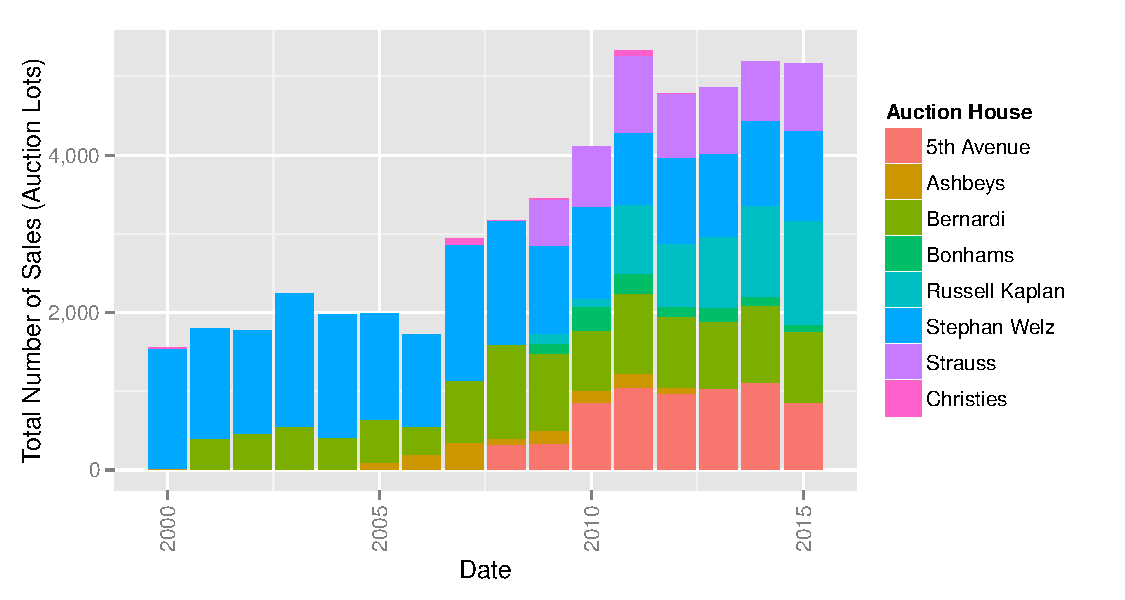
\includegraphics{Art_Price_Indices_3_files/figure-latex/figure1-1.pdf}
\caption{Total Number of Auction Lots Sold by auction house (2000-2015)}
\end{figure}

Figure 2 illustrates boxplots for the logarithm of the hammer prices for
each year. The sample is highly positively skewed, with the overall mean
price of R49,824 much higher than the median of R7,000. There were a
number of outliers, including the hammer price of over R30 million for
Irma Stern's \emph{``Arab Priest''} in 2011. Annual median sales prices
increased substantially from R3,200 in 2003 to R10,000 at its peak in
2010. This confirms anecdotal evidence on the rise in popularity of the
South African art market.

\begin{figure}[htbp]
\centering
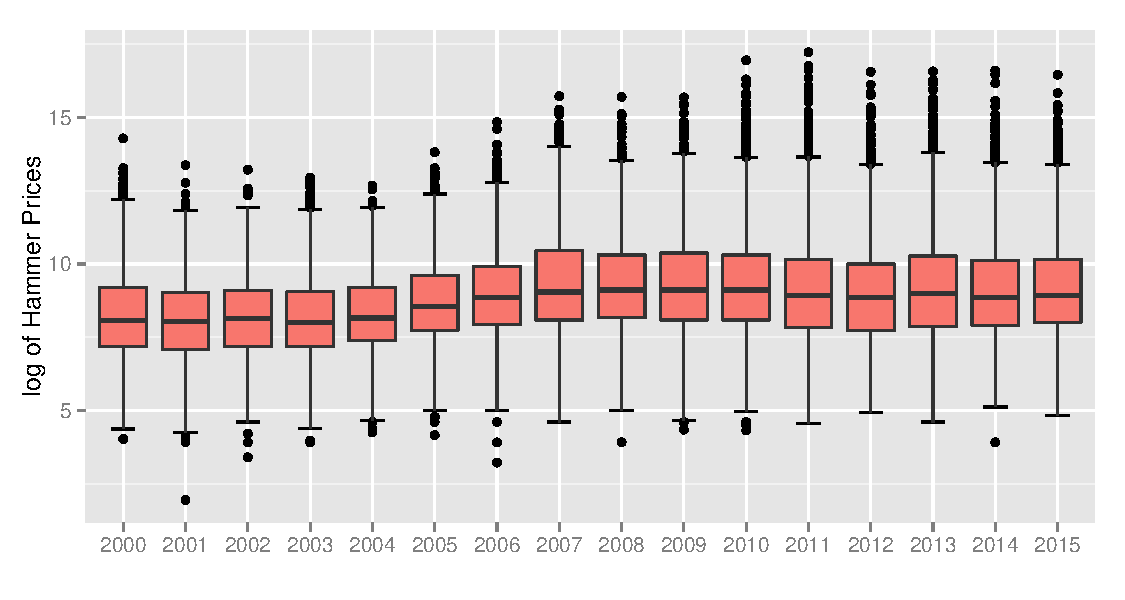
\includegraphics{./tex2pdf.15156/5dc54430024651a97e1e9f01cc30cdef606939f9.pdf}
\caption{Boxplot of the logarithm of hammer prices}
\end{figure}

\subsection{Artwork characteristics}\label{artwork-characteristics}

Hedonic art price models typically include characteristics that are
relatively easily observable and quantifiable. This section briefly
discusses the variables typically included in hedonic models of art
prices.

\emph{Artist reputation}: Hedonic models typically include dummy
variables to control for the artists. However, some artists often have
to be excluded from estimation, due to a lack of degrees of freedom.
Alternatively, a reputation variable can be constructed, either from the
art literature, or from the auction data itself with a procedure like
the 2-step hedonic approach suggested by Kräussl and Van Elsland (2008).
The models in this paper are estimated using a continuous reputation
variable, as explained below.

\emph{Size}: The most common variable used to describe the physical
characteristics of an artwork is its size or surface area. The models
use the natural logarithm of the surface area of the artwork in
\(cm^2\). The models also include an interaction term for sculpture
size, as the size of a sculpture is usually only recorded in terms of
its height (in cm). Figure 3 illustrates the positive relationship
between artwork sizes and prices, by medium. Squared values are
occasionally included to take potential non-linearities into account
(Fedderke and Li, 2014). In this sample, however, the relationship does
not seem to exhibit an inverted U-shape and the squared term is positive
and economically insignificant in the regression models.

\begin{figure}[htbp]
\centering
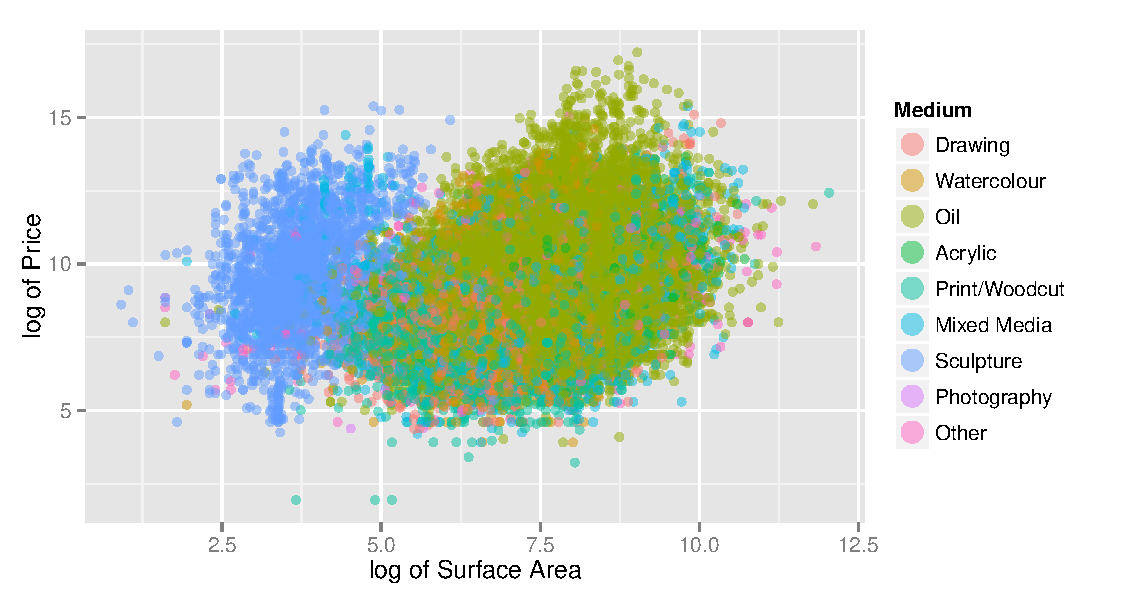
\includegraphics{Art_Price_Indices_3_files/figure-latex/figure3-1.pdf}
\caption{Relationship between prices and artwork sizes, by medium}
\end{figure}

\emph{Auction house}: Dummy variables for the auction houses are also
typically included. The more prominent auction houses usually have a
positive effect on prices. One reason might be that the more renowned
auction houses will offer higher quality work (Kräussl and Logher,
2010). Thus, the variables might be picking up otherwise unobservable
quality differences and do not necessarily reflect auction house
certification (Renneboog and Spaenjers, 2013). Moreover, different
auction houses charge different commissions to both buyers and sellers.
For example, Strauss \& Co reported a buyer's premium of 10\%-15\%,
while Bonhams charged premiums of up to 25\% (Olckers, Kannemeyer and
Stevenson, 2015). The hammer prices exclude these premiums and are
therefore not a perfect measure of the cost to the buyer and revenue to
the seller. For the purposes of a price index the auction house dummies
should capture the different premiums charged by the auction houses.

\emph{Mediums}: Average prices vary across mediums. This might be due to
the durability of the medium, the stage of production the medium is
associated with (e.g.~preparatory drawings) and in some case the
replacement value of the materials used (e.g.~sculptures cast in
bronze). Oil paintings traditionally earn the highest prices. The
availability of copies may decrease the prices of prints and photographs
relative to other mediums. Studies typically include dummy variables for
the different mediums as defined in their data (Kräussl and Logher,
2010). The models in this section use the 9 mediums defined in the
dataset; the same mediums used by Olckers, Kannemeyer and Stevenson
(2015).\footnote{The data do not include enough detail to differentiate
  between medium (e.g.~oil) and material (e.g.~canvas), or to identify
  the subject matter or theme of an artwork (e.g.~portraits, landscapes,
  abstract works). A few studies have included dummies to indicate
  whether an artist was alive. Artworks of artists who are no longer
  alive are generally thought to be more valuable, as the production has
  ceased. However, artists who are no longer alive are not able to build
  on their reputation, which might result in lower sale prices in the
  long run (Kräussl \& Lee 2010). Hence, it is not clear if the variable
  will be significant. Fedderke \& Li (2014) found that the date of
  death and age of the artist were statistically insignificant for their
  South African sample.}

\emph{Authenticity dummies}: Models often include dummies for whether
the artwork is signed and dated. There might be a premium for these
attributes, as there is less uncertainty about authenticity (Renneboog
and Spaenjers, 2015). These dummies are included in the models below and
are expected to have positive coefficients.

\emph{Number of works in the lot}: The models below also control for
cases in which more than one artwork was sold in the same auction lot.
This is because the recorded size corresponded to each artwork
separately and not the group. Moreover, it is possible that lots
including more than one artwork fetch a lower price per artwork than if
they sold separately.

\emph{Date dummies}: The models below include time dummies at a
quarterly frequency, which are used to estimate the indices. The
exponentials of the time dummy coefficients represent the appreciation
in the value of art in that specific period, relative to the common base
period.\footnote{Such an index will track the geometric mean, rather
  than the arithmetic mean, of prices over time, because of the log
  transformation prior to estimation. If it is assumed that the
  regression residuals are normally distributed in each period, a
  correction can be made by defining corrected index values as:
  \(I_t =\exp\left[\gamma_t+ 1/2(\sigma_t^2-\sigma_0^2 )\right]*100\),
  where \(\sigma_t^2\) is the estimated variance of the residuals in
  period t (Renneboog \& Spaenjers 2012). In practice this adjustment is
  often negligible (Hansen 2009), which is also the case in this sample.}

\subsubsection{Continuous artist reputation variable: two-step hedonic
approach}\label{continuous-artist-reputation-variable-two-step-hedonic-approach}

The number of artist dummy variables that can be included in the hedonic
regression is limited by the degrees of freedom, which means that some
artists usually get excluded from the sample. Kräussl and Van Elsland
(2008) developed a two-step hedonic approach, which allows the use of
every auction record, instead of only those auction records that belong
to a sub-sample of selected artists. The approach involves the
estimation of a continuous artist reputation variable, which is included
in the regression instead of the artist dummy variables. In this way the
approach increases the sample size of artworks that can be included in
the regression models and reduces selection bias.

Triplett (2004) showed that a hedonic function with a logarithmic
dependent variable would yield an index equal to the ratio of the
unweighted geometric means of prices in periods \(t\) and \(t+1\),
divided by a hedonic quality adjustment. The superscripts \(n\) and
\(m\) indicate the generally unequal number of artworks sold per period.
The hedonic quality adjustment is a quantity measure of the mean change
in the \(j\) characteristics of items sold in period \(t\) and \(t+1\),
valued by their implicit prices (\(\beta_j\)):
\[Index = \frac{\prod_{i=1}^n (P_{i,t+1})^\frac{1}{n}} {\prod_{i=1}^m (P_{i,t})^\frac{1}{m}} / \text{hedonic adjustment} \]
\[\text{hedonic adjustment} = \exp \left[\sum_{j=1}^J\beta_j(\sum_{i=0}^n \frac{X_{ji,t+1}}{n}- \sum_{i=1}^m \frac{X_{ji,t}}{m})\right]\]

Kräussl and Van Elsland (2008) argued that the same method could be used
to adjust the average price of an artist's work for differences in
quality. The resulting index yields the value of artworks by artist
\(y\), relative to the base artist \(0\):
\[\text{Artist reputation index} = \frac{\prod_{i=1}^n (P_{i,y})^\frac{1}{n} / \prod_{i=1}^m (P_{i,0})^\frac{1}{m}} {\exp \left[\sum_{j=1}^z \beta_j(\sum_{i=0}^n \frac{X_{ji,y}}{n} - \sum_{i=1}^m  \frac{X_{ji,0}}{m}) \right]} \]

where \(P_{i,y}\) is the value of painting \(i\) \((i=0,..., n)\),
created by artist \(y\); \(X_{ji}\) are the characteristics of the
artworks, excluding the artist dummy variables.

The first step is to estimate the full hedonic model on a sub-sample of
artists to obtain the characteristic prices (\(\beta_j\)). Following
Kräussl and Van Elsland (2008), the sub-sample includes the top 100
artists in terms of volume, representing 53\% of records and 92\% of the
value in the sample. The coefficients are similar to those for the full
pooled model and it is assumed that the characteristic prices are
representative. In the second step, the artist reputation index is
calculated for each artist relative to the base artist (Walter Battiss),
i.e.~the relative quality-corrected prices for the works of artist \(y\)
relative to artist \(0\). The reputation index is then used as a
continuous proxy variable for artistic value in the hedonic models,
instead of the artist dummies.

Figure 4 illustrates the positive relationship between artwork prices
and the reputation index. As a robustness check, the models are also
estimated including all of the artist dummies, except for those artists
that only sold one artwork over the sample period. The results were very
similar, in line with the findings in Kräussl and Van Elsland (2008).

\begin{figure}[htbp]
\centering
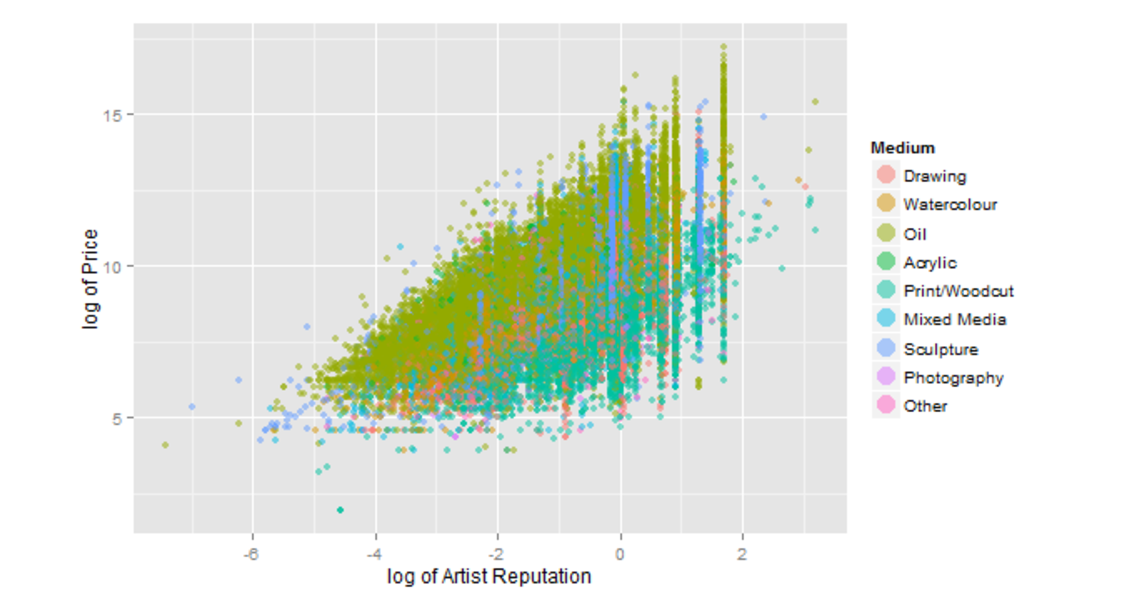
\includegraphics{Art_Price_Indices_3_files/figure-latex/figure4-1.pdf}
\caption{Relationship between prices and reputation index}
\end{figure}

\section{Results}\label{results}

\subsection{Central Tendency Indices}\label{central-tendency-indices}

Two central tendency price indices are estimated at a quarterly
frequency to act as a baseline in comparing the indices resulting from
the different methodologies. The median index is simply the median price
for each quarter. The Fisher index is a mix-adjusted central tendency
index, which is stratified by artist and medium. The base periods are
allowed to vary for each index point and the index points are then
chained together to form the overall chain-link index.

Figure 5 illustrates the two central tendency indices. The simple median
index provides a noisy estimate of price changes and no consistent
picture emerges. The large variation is likely due to the large
differences in quality-mix or composition of the artworks sold between
different periods.

\begin{figure}[htbp]
\centering
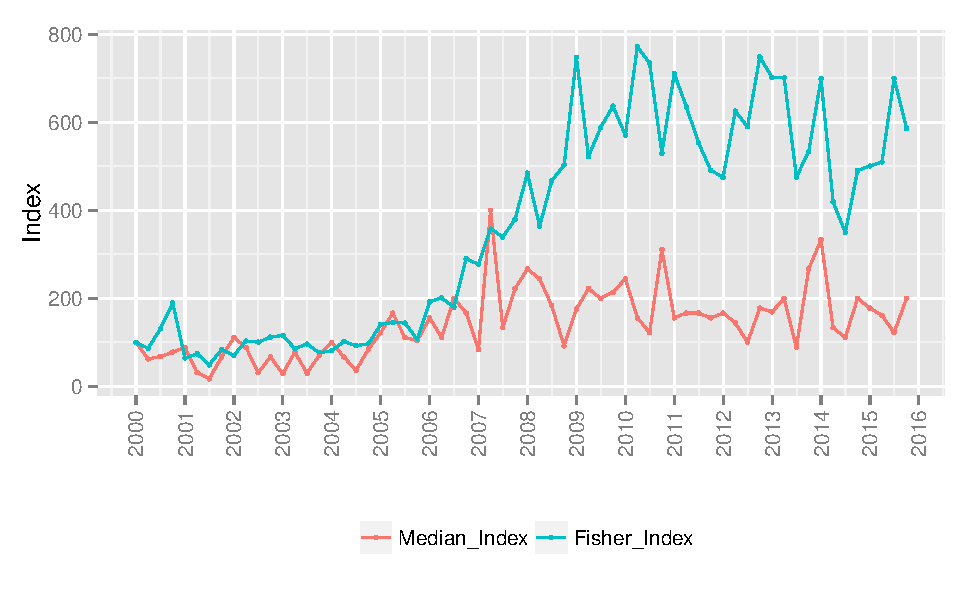
\includegraphics{Art_Price_Indices_3_files/figure-latex/figure5-1.pdf}
\caption{Central tendency South African art price indices (2000Q1=100)}
\end{figure}

The Fisher index also exhibits a large variation and implausibly large
increases over the sample period. In this case the stratification does
not seem to be very effective. This is probably because the artist and
medium categories only capture a small portion of the differences in the
quality of artworks that come to market between periods. The
mix-adjusted measure will not account for any changes in the mix of
artworks sold that are unrelated to artist and medium type. The
stratified index also does not account for changes in the mix of
artworks sold within each subgroup, in this case changes in the mix of
artworks by a certain artist in a specific medium (Eurostat, 2013).
Moreover, the subgroups become small when separated in this way, which
means that small changes can have a large effect on the index.

The results illustrate that central tendency measures are deficient in
this case and should be used with caution, confirming the findings in
Els and Von Fintel (2010). As a consequence, regression-based measures
are generally preferred in the academic literature. The hedonic indices
in the following section control for quality changes by taking many more
of the artwork attributes into account.

\subsection{Hedonic Indices}\label{hedonic-indices}

The full pooled sample estimation results are reported in Table 1. The
coefficients are all significant and have the expected signs. The size
of the artwork is highly significant and positive, as is the sculpture
interaction term. Bonhams and Strauss \& Co are the auction houses with
the highest average prices, after controlling for other factors,
probably reflecting higher quality work and higher commission
structures. Oil is the most expensive medium category. The
authentication dummies are both positive and significant, as is the
artist reputation variable. The number of works dummy indicates that
more than one artwork in a lot leads to slightly lower prices per
artwork. The adjusted \(R^2\) is relatively high, suggesting that these
variables capture a relatively large part of the variation in sales
prices.\footnote{The diagnostic tests indicate that there might be some
  problems with the assumptions of normality and homoscedasticity of the
  residuals. These assumptions are not crucial, however, as only the
  point estimates of the time dummy coefficients are of interest.} The
time dummy coefficients are then used to calculate the full period
pooled hedonic index.

\begin{table}[!h] \centering 
  \caption{Hedonic Regression results} 
  \label{} 
\begin{tabular}{@{\extracolsep{5pt}}lc} 
\\[-1.8ex]\hline 
\hline \\[-1.8ex] 
 & \multicolumn{1}{c}{\textit{Dependent variable:}} \\ 
\cline{2-2} 
\\[-1.8ex] & lnprice \\ 
\hline \\[-1.8ex] 
 lnarea & 0.405$^{***}$ (0.004) \\ 
  ah\_codeAshbeys & 0.114$^{***}$ (0.028) \\ 
  ah\_codeBernardi & 0.122$^{***}$ (0.013) \\ 
  ah\_codeBonhams & 1.198$^{***}$ (0.026) \\ 
  ah\_codeChristies & 1.152$^{***}$ (0.065) \\ 
  ah\_codeRussell Kaplan & 0.129$^{***}$ (0.015) \\ 
  ah\_codeStephan Welz & 0.590$^{***}$ (0.013) \\ 
  ah\_codeStrauss & 1.126$^{***}$ (0.016) \\ 
  med\_codeWatercolour & 0.553$^{***}$ (0.017) \\ 
  med\_codeOil & 1.435$^{***}$ (0.014) \\ 
  med\_codeAcrylic & 1.039$^{***}$ (0.033) \\ 
  med\_codePrint/Woodcut & $-$0.759$^{***}$ (0.015) \\ 
  med\_codeMixed Media & 0.554$^{***}$ (0.017) \\ 
  med\_codeSculpture & 1.767$^{***}$ (0.084) \\ 
  med\_codePhotography & $-$0.618$^{***}$ (0.085) \\ 
  med\_codeOther & 0.703$^{***}$ (0.035) \\ 
  lnsculpt\_area & 0.236$^{***}$ (0.021) \\ 
  dum\_signed & 0.208$^{***}$ (0.016) \\ 
  dum\_dated & 0.045$^{***}$ (0.007) \\ 
  nr\_works & $-$0.096$^{***}$ (0.003) \\ 
  lnrep & 0.949$^{***}$ (0.003) \\ 
  Constant & 5.101$^{***}$ (0.065) \\ 
 \hline \\[-1.8ex] 
Quarterly dummies & Yes \\ 
\hline \\[-1.8ex] 
Observations & 51,454 \\ 
R$^{2}$ & 0.782 \\ 
Adjusted R$^{2}$ & 0.782 \\ 
Residual Std. Error & 0.780 (df = 51369) \\ 
F Statistic & 2,196.018$^{***}$ (df = 84; 51369) \\ 
\hline 
\hline \\[-1.8ex] 
\textit{Note:}  & \multicolumn{1}{r}{$^{*}$p$<$0.1; $^{**}$p$<$0.05; $^{***}$p$<$0.01} \\ 
\end{tabular} 
\end{table}

To allow for shifts the implicit prices, two adjacent-period or
chain-linked indices are calculated by estimating separate models for
adjacent sub-samples. There is a trade-off in selecting the length of
the estimation window. Shorter estimation windows decrease the
likelihood of large breaks but also decrease the number of observations
used to estimate the parameters (Dorsey \emph{et al.}, 2010). 1-year and
2-year estimation windows are selected, similar to Dorsey \emph{et al.}
(2010) in the context of real estate and Renneboog and Spaenjers (2013)
in the context of art. This seems to be reasonable for the South African
art market, where large auctions are held relatively infrequently. The
indices are then calculated by chain-linking the estimates together, as
Figure 6 illustrates for the 2-year version of the index.

\begin{figure}[htbp]
\centering
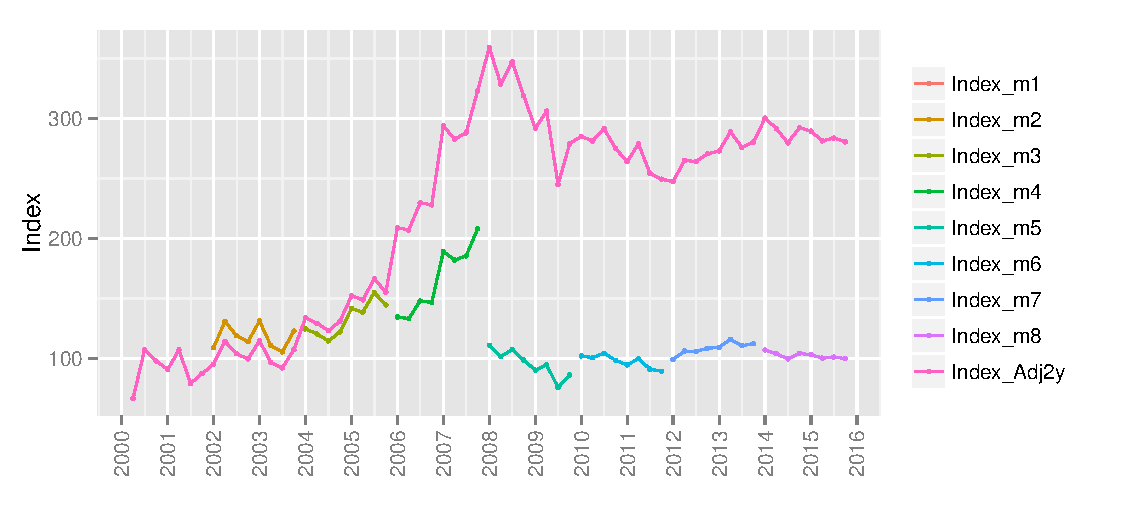
\includegraphics{Art_Price_Indices_3_files/figure-latex/figure6-1.pdf}
\caption{Chain-linked two-year adjacent period art price index}
\end{figure}

In the context of real estate, Shimizu, Nishimura and Watanabe (2010)
suggested a so-called overlapping-periods hedonic regression method
using multiple ``neighbourhood periods'', allowing gradual shifts in the
parameters. Parameters are estimated by taking a certain length as the
estimation window and shifting the period forward in rolling
regressions. They argued that this method should be able to handle
seasonal changes in parameters better than adjacent-periods regressions,
although it may suffer more from the disadvantages associated with
pooling. To apply this method, 5-year rolling regressions were run,
which corresponds to the rolling 5-year regressions used to estimate the
Citadel Art Price Index. The estimation window is then shifted forward
one year, allowing for gradual shifts in the parameters.

The coefficients from these models are similar in magnitude to the full
pooled sample model and significant in virtually all cases. For example,
the coefficient associated with the size of the artwork is 0.426 using
the standard hedonic regression, while the average coefficients from the
other regressions are 0.44, 0.43 and 0.42. However, there are a few
cases in which the estimated parameters fluctuate quite substantially.
For example, the coefficient of the Strauss auction house dummy varies
between 1.04 in the pooled model and 0.77 in one the sub-samples,
indicating that non-negligible structural changes might have occurred
during the sample period.

Figure 7 illustrates the resulting quarterly art price indices from
these four models. The hedonic indices follow a similar cyclical pattern
over the period, although the levels are slightly different, and
appreciated rapidly in the run-up to the Great Recession. The indices
seem more plausible than the central tendency measures, supporting the
case for regression-based measures.\footnote{Two additional hedonic
  model extensions were performed as a robustness test: stratified
  hedonic indices by medium and quantile hedonic indices. The results
  are very similar to the results reported above.} All four of the
indices peak in 2008Q1, which is before the peak in sales and annual
median prices in the sample. All four of the indices displayed dramatic
increases in auction prices of more than 200\% between 2003 and 2008.
This conforms to the idea that there was a surge in the popularity of
South African art over the period, as well as the idea of the formation
of a so-called bubble, with a dramatic rise and subsequent decrease in
prices.

\begin{figure}[htbp]
\centering
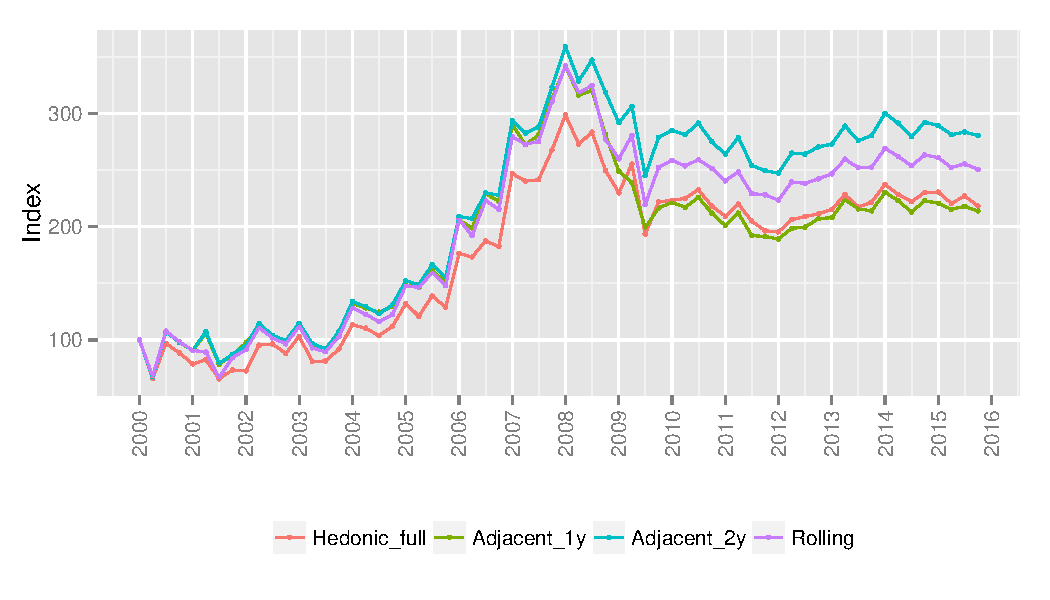
\includegraphics{Art_Price_Indices_3_files/figure-latex/figure7-1.pdf}
\caption{Hedonic South African art price indices (2000Q1=100)}
\end{figure}

The hedonic price indices display similar trends over the period, with
large price increases in the run-up to the Great Recession. However, the
hedonic indices may suffer from omitted variable or misspecification
bias. Ramsey RESET tests indicate that the models might be misspecified.
The omitted variables might include unobservable (or difficult to
measure) nuances that make a given artwork unique and influence its
price. The omitted variables might include, for instance, interaction
terms (e.g.~artist and medium combinations), squared terms, finer medium
classifications (e.g.~a specific artist's Print/Woodcuts might typically
be linocuts), or attributes such material, theme and style (e.g.~a
specific artist's oil paintings might typically use the same material
such as canvas, or have the same theme such as a portrait). These
omitted variables potentially bias the coefficients if they are
correlated with sales timing, which in turn may bias the indices,
although the bias is often small in practice (Triplett, 2004; Renneboog
and Spaenjers, 2013).

The following section estimates alternative art price indices using a
hybrid repeat sales methodology, which should be less prone to omitted
variable bias. If the alternative indices displays the same kind of
trend and the same marked increase in prices as the hedonic indices,
this should provide more confidence that the results are robust to
changes in methodology and that omitted variable bias is not driving the
results.

\subsection{Repeat Sales and Hybrid
Indices}\label{repeat-sales-and-hybrid-indices}

The repeat sales method is less prone to potential omitted variable bias
than the hedonic method, as it tracks the sales of the same item over
time. Because the dataset does not uniquely identify each artwork,
repeat sales of the same artwork were identified by matching sales
records using the following hedonic attributes: artist name, artwork
title, size, and medium, the presence of a signature and a date, and the
number of artworks in the lot. Only 515 true repeat sales pairs could be
identified in the sample. Figure 8 illustrates the index generated using
the classical repeated sales approach. The index is volatile, with many
missing values, and exhibits a large appreciation in prices over the
period. The limited number of repeat sales observations therefore limits
the usefulness of the classical repeated sales approach in this case.

\begin{figure}[htbp]
\centering
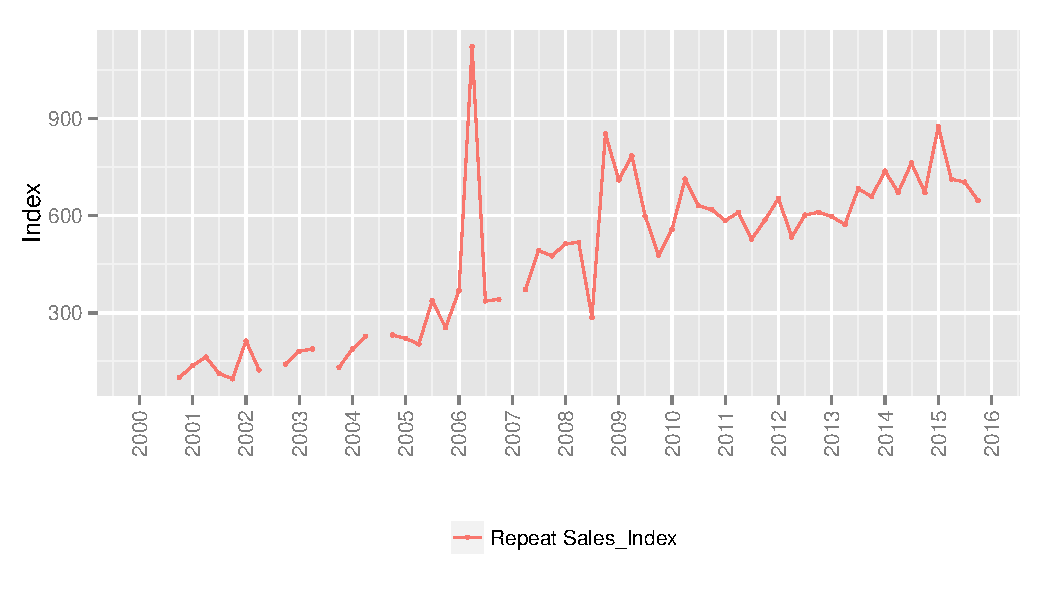
\includegraphics{Art_Price_Indices_3_files/figure-latex/figure8-1.pdf}
\caption{Repeat sales index of South African art prices (2000Q4=100)}
\end{figure}

As an alternative the paper proposes the application of a simple hybrid
repeat sales model to art prices for the first time. This procedure is
similar in spirit to the ``pseudo repeat sales'' (ps-RS) procedure
suggested by Guo \emph{et al.} (2014). Instead of requiring an exact
match to form a sales pairs, very similar artworks may be treated as
repeat sales pairs. In this way the ps-RS method supplements the true
repeat sales in the sample and mitigates the problem of small sample
size. In so doing it allows the estimation of a variant of the repeat
sale index, which should address to some extent the potential omitted
variable bias inherent in the hedonic method. The caveat is that even
two artworks by the same artist of a similar size and in the same medium
do not necessarily serve as close substitutes (Olckers, Kannemeyer and
Stevenson, 2015).

The first ps-RS sample is created by matching artworks on all the
hedonic attributes, except the title of the artwork. The matched pairs
therefore have the same hedonic attributes except for the title of the
artwork. Matching by this criteria increases the number of repeat sales
pairs to 6,642, which includes the 515 true repeat sales or exact
matches. The second ps-RS sample allows the sample to increase further
by matching on all the hedonic attributes except the title and the
presence of a signature and a date on the artwork, i.e.~the authenticity
dummies. This increases the pseudo repeat sales sample to 7,965 sales
pairs. This procedure involves a trade-off between the within-pair
``similarity'' (higher similarity is good for mitigating bias) and the
sample size (larger size is good for reducing random errors).

The differential hedonic equation is then applied to the pseudo repeat
sales samples, where artwork \(i\) in quarter \(t\) and artwork \(h\) in
quarter \(s\) form a matched pair \((t>s)\):
\[\ln P_{it} - \ln P_{hs} = \sum_{j=1}^J \beta_j (X_{itj} - X_{hsj}) + \sum_{t=0}^T \delta_t G_{it} + \epsilon_{iths}\]
where \(G_{it}\) is again a time dummy equal to 1 if the later sale
occurred in quarter \(t\), -1 if the former sale in the pair occurred in
quarter \(s\), and 0 otherwise; and \(\epsilon_{iths}\) again represents
a white noise residual.

For the first ps-RS sample, the only remaining independent variable is
the difference in the auction house dummies \((X_{it1} - X_{hs1})\).
This takes account of possible differences in quality and commission
structures. In the second ps-RS sample the independent variables
represent the differences in the auction house dummies and the
differences in the two authenticity dummies. The independent variables
therefore include indicators of the relatively small and easy to measure
within-pair differentials in attributes between the two items.

Thus, the ps-RS approach addresses the problem of lack of repeat sales
data and to some extent the potential omitted variable bias inherent in
the hedonic method. The pseudo repeat sales pairs include the 515 true
repeat sales, or exact matches, where the model controls for all the
observed and unobserved attributes by taking first differences. For the
pseudo sales pairs, taking first differences will control for omitted
variables when they are the same for the two items that form the pseudo
sales pairs. For example, if Van Gogh's \emph{Sunflowers} paintings are
treated as repeat sales, taking first differences would control for
attributes such as theme, style, material, prominence, and the stage of
the artist's career. Other potentially significant variables might
include an array of interaction and non-linear terms.

Figure 9 illustrates the two versions of the ps-RS indices. The indices
point to similar cyclical trends in art prices over the sample period,
although the ``purest'' pseudo repeat sales index is at a higher level
than the other index. The larger sample appears to reduce the volatility
of the index, which is similar to the findings in Guo \emph{et al.}
(2014). Both indices appreciated rapidly in the run-up to the Great
Recession and peaked in 2008Q1. The indices point to the same kind of
marked increase in South African art prices as the hedonic indices,
which provides more confidence that the results are robust to changes in
methodology. The following section further compares and evaluates the
different art price indices.

\begin{figure}[htbp]
\centering
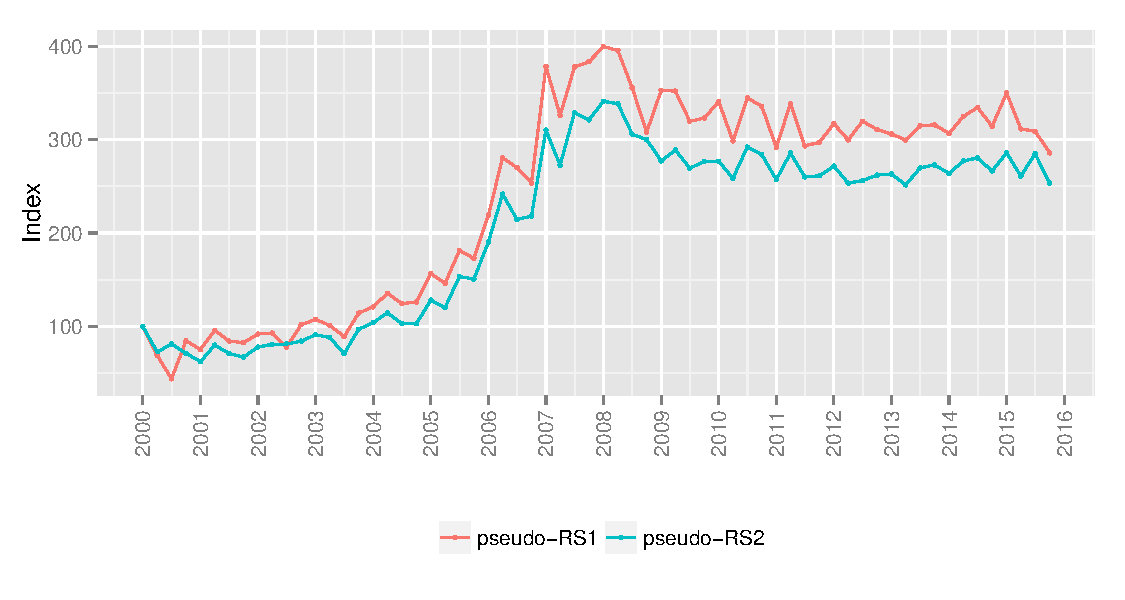
\includegraphics{Art_Price_Indices_3_files/figure-latex/figure9-1.pdf}
\caption{Pseudo repeat sales South African art price indices
(2000Q1=100)}
\end{figure}

\section{Comparison and Evaluation}\label{comparison-and-evaluation}

This section compares the different art price indices in order to
determine if they provide a consistent picture of price movements in the
South African art market. The indices are evaluated in terms smoothness
to examine which index provides the most credible gauge of overall price
movements in this specific case. The art price indices are also compared
to available international art price indices and other South African
assets over the sample period, to check if the results are reasonable.

\subsection{Comparison of the indices}\label{comparison-of-the-indices}

The art price indices are first compared graphically. Figure 10
illustrates representative indices for the three methodologies: median
values, the 2-year adjacent period hedonic index and the second version
(larger sample) of the ps-RS index. The two regression-based indices
seem to point to a similar general trend in South African art prices.
The simple median index, on the other hand, does not reflect this trend
and is much more volatile than the regression-based indices. This
implies that regression-based methods, which adjust for changes in the
composition or quality-mix of artworks sold, provide better estimates of
pure price changes for unique assets. The results confirm the findings
for South African real estate in Els and Von Fintel (2010).

\begin{figure}[htbp]
\centering
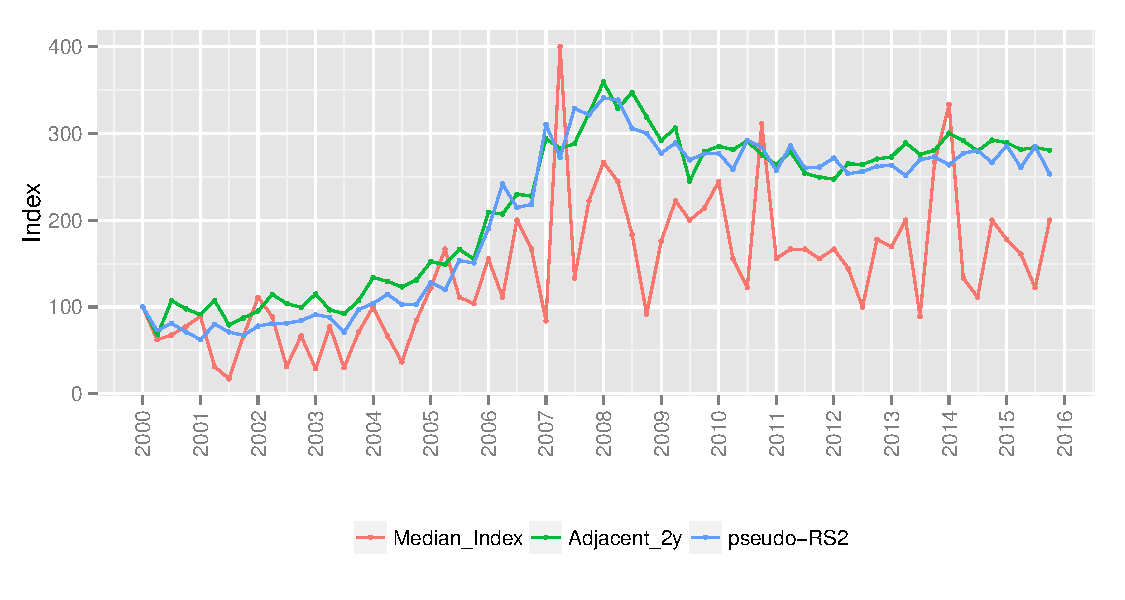
\includegraphics{Art_Price_Indices_3_files/figure-latex/figure10-1.pdf}
\caption{Comparing South African art price indices (2000Q1=100)}
\end{figure}

The hedonic and ps-RS indices exhibit remarkably similar trends over the
sample period. Both measures indicate that the average price of a
constant-quality artwork increased significantly between 2005 and 2008
and then declined relatively sharply after the financial crisis, similar
to other asset prices (Shimizu, Nishimura and Watanabe, 2010). The fact
that the regression-based indices are similar, even when the hybrid
repeat sales indices are based on smaller subsamples of the data,
implies that the potential omitted variable and sample selection bias
may not be too pervasive in this case. The ps-RS method provides a type
of robustness check on the hedonic indices.

Table 2 reports the correlations in the growth rates between the various
indices.\footnote{The first few periods of repeat sales estimates are
  often sensitive when the sample size is small, because of the lack of
  repeat sales in the first few quarters. In this case very few artworks
  had been resold in the few three quarters, making the index values
  very volatile. Indeed there are no true repeat sales in the first
  three quarters of the sample period. The first three index values were
  therefore excluded from the comparison.} There is a significant
positive correlation between the regression-based indices. This
indicates that their general trends are similar, and are different from
the simple median. The Fisher central tendency index is also
significantly positively correlated with the hedonic indices. This shows
that there is some consistency in the estimates from the different
methodologies, which provides some confidence that the indices provide a
relatively accurate measure of the price movements in the South African
art market. The following section compares the indices more formally by
evaluating index smoothness.

\begin{table}[ht]
\centering
\caption{Correlations in growth rates (dlogs)} 
\scalebox{0.9}{
\begin{tabular}{rllllllll}
  \hline
 & Median & Fisher & Hedonic & Adj1y & Adj2y & Roll & RepSale & ps.RS1 \\ 
  \hline
Median &  &  &  &  &  &  &  &  \\ 
  Fisher &  0.13  &  &  &  &  &  &  &  \\ 
  Hedonic &  0.03  &  0.40**  &  &  &  &  &  &  \\ 
  Adj1y &  0.11  &  0.35**  &  0.90*** &  &  &  &  &  \\ 
  Adj2y &  0.11  &  0.38**  &  0.94*** &  0.98*** &  &  &  &  \\ 
  Roll &  0.23  &  0.38**  &  0.94*** &  0.94*** &  0.95*** &  &  &  \\ 
  RepSale &  0.20  &  0.00  & -0.11  & -0.07  & -0.03  & -0.11  &  &  \\ 
  ps.RS1 & -0.01  &  0.08  &  0.48*** &  0.58*** &  0.56*** &  0.47*** &  0.12  &  \\ 
  ps.RS2 & -0.16  &  0.08  &  0.52*** &  0.59*** &  0.58*** &  0.46*** &  0.23  &  0.87*** \\ 
   \hline
\end{tabular}
}
\end{table}

\subsection{Comparative Performance of the Art Price
Indices}\label{comparative-performance-of-the-art-price-indices}

The next step is to evaluate the comparative performance of the indices
produced with the different methodologies. This is not usually attempted
for art price indices, given that most papers focus on a specific
method. In other applications, the quality of price indices has often
been evaluated based on the diagnostic metrics of the underlying
regressions, such as the standard errors of the residuals (see e.g.
Hansen (2009) for real estate indices).

However, Guo \emph{et al.} (2014) argued that the regression residuals
do not represent errors in the price index, and hence do not directly
reflect inaccuracy in the index returns. Even if an index is perfectly
accurate, measuring the central tendency of market price changes in each
period, the regression would still have residuals and the time dummy
coefficients might still have large standard errors, resulting simply
from the dispersion of individual art prices around the central
tendency. When datasets become large, the regression diagnostics are
often impressively good simply because of the size of the sample. In
such cases, tests of economic significance are more valuable than tests
of statistical significance. Moreover, in this case not all of the
indices are generated with regression models. The regressions models
that are employed differ in their specifications (in levels or first
differences) and the underlying data sets used for estimation.

Guo \emph{et al.} (2014) suggested that signal-to-noise metrics, based
directly on the index produced, are a more appropriate for judging the
quality of the price index, as opposed to the underlying model. Random
error in the coefficient estimation leads to ``noise'' in the index.
Signal-to-noise metrics directly reflect the accuracy of the index
returns and the economic significance of random error in the indices.
The volatility (Vol) and the first order autocorrelations (AC(1)) of the
index returns are signal-to-noise metrics that may be useful to compare
the amount of noise in the indices.

Consider the simple model of random noise in the index:
\[m_t=m_{t-1}+r_t\] and
\[I_t=m_t+\epsilon_t=\sum_{i=1}^tr_i+\epsilon_t\] where \(m_t\) is the
true market value level (in logs); \(r_t\) is the true return (i.e.~the
central tendency) of market prices in period \(t\); \(I_t\) is the index
in period \(t\); \(\epsilon_t\) is the index-level random (white noise)
error. This random error causes noise in the index and therefore matters
from the perspective of index users. The noise does not accumulate over
time.

The index returns can be defined as follows:
\[r_t^*=I_t-I_{t-1}=r_t+(\epsilon_t-\epsilon_{t-1})= r_t+\eta_t\] where
\(r_t^*\) is the index return and \(\eta_t\) is the noise component of
the index return in period \(t\).

The volatility of the index (Vol), which is the standard deviation of
the index return \(\sigma_{r_t^*}\) and the first order autocorrelation
\(\rho_{r^*}\) (AC(1)) can be derived as:
\[Vol = \sigma_{r_t^*} = \sqrt{\sigma_r^2 + \sigma_\eta^2}\] and
\[AC(1) = \rho_{r^*} = (\rho_r \sigma_r^2 - \sigma_\eta^2/2) / (\sigma_r^2 + \sigma_\eta^2)\]
where \(\sigma_r^2\) and \(\sigma_\eta^2\) are the variance of the true
return and the noise respectively, and \(\rho_r\) is the first order
autocorrelation coefficient of the true return.

Volatility is the dispersion in returns over time. There is always true
volatility as the true market prices evolve over time. The ideal price
index filters out the noise-induced volatility to leave only the true
market volatility. In addition to the true volatility, the noise (random
error) in the index causes excess volatility in the index returns.
Excess volatility decreases the first order autocorrelation in index
returns. Less noise (lower \(\sigma_\eta^2\)) will lead to lower index
volatility and higher AC(1). Other things being equal, the lower the
volatility and the higher the AC(1), the less noisy and more accurate
the index. Thus, lower Vol or higher AC(1) will indicate a better
quality art price index in the sense of less noise.

Guo \emph{et al.} (2014) suggest another test of index quality in terms
of minimising random error that is based on the Hodrick-Prescott (HP)
filter. The HP filter is a spline fitting procedure that divides a time
series into smoothed trend and cyclical components. The idea is to
examine which index has the least deviation from its smoothed HP
component, by comparing the sum of squared differences between the index
returns and the smoothed returns.

Another option is to compare the smoothness coefficients proposed by
Froeb and Koyak (1994). The smoothness coefficient is defined as the
average long run variance of a time series divided by the average short
run variance. The idea is to obtain the spectral density of the time
series, which shows the contribution of all frequencies to the data
series. The smoothness measure is then taken as the average of the lower
half of the frequency range (i.e.~the low frequency or longer term
movements) over the average of the upper half of the frequencies
(i.e.~the higher frequencies or shorter term). In other words, the
smoothness coefficient is the low frequency portion divided by the high
frequency portion of the periodogram.\footnote{The spectral density is
  smoothed using the Daniell window, which amounts to a simple moving
  average transformation of the periodogram values.} A higher smoothness
coefficient indicates a larger portion of variance in the low
frequencies and a smoother time series.

Table 3 reports these four metrics of index smoothness for the art price
indices. The comparison suggests that that the regression-based indices
are much smoother than the central tendency measures and the classical
repeat sales index. The volatilities, autocorrelations and HP filter
deviations of the regression-based indices are around the same size. The
larger sample ps-RS index performs the best in terms of these three
metrics, with lower volatility and higher AC(1) in returns, and a
smaller deviation from its smoothed returns. According to the smoothness
coefficient, the hedonic indices perform the best and the 1-year
adjacent period hedonic index exhibits the highest smoothness
coefficient. However, the smoothness coefficients of the
regression-based indices are not significantly different statistically.

\begin{table}[ht]
\centering
\caption{Smoothness Indicators} 
\scalebox{0.9}{
\begin{tabular}{rrrrr}
  \hline
 & Vol & AC.1 & HPDeviation & Smoothness \\ 
  \hline
Median & 0.606 & -0.414 & 22.34 & -0.02 \\ 
  Fisher & 0.296 & -0.477 & 5.24 & 1.00 \\ 
  Hedonic & 0.130 & -0.394 & 1.00 & 1.14 \\ 
  Adj1y & 0.126 & -0.342 & 0.93 & 1.54 \\ 
  Adj2y & 0.126 & -0.394 & 0.95 & 1.17 \\ 
  Roll & 0.131 & -0.364 & 1.02 & 1.36 \\ 
  RepSale & 0.444 & -0.408 & 12.01 & 0.58 \\ 
  ps.RS1 & 0.135 & -0.390 & 1.10 & 0.79 \\ 
  ps.RS2 & 0.124 & -0.285 & 0.92 & 0.86 \\ 
   \hline
\end{tabular}
}
\end{table}

\subsection{Comparing the art price indices to other asset
prices}\label{comparing-the-art-price-indices-to-other-asset-prices}

To check that the estimated South African art price indices provide
reasonable results, they can be compared to available international art
price indices and other South African assets over the sample period.

Figure 11 illustrates the art price indices for the US, UK and France,
calculated by Artprice, together with two representative South African
art price indices. In contrast to the other art price indices, the South
African art market index experienced a decrease at the start of the
period. All of the art price indices increased substantially between
2005 and 2008, although the South African art price indices exhibited
higher growth rates. The Top 500 Art Market index in Kräussl and Lee
(2010) also reflects this trend, with a sharp decline in 2008, which
they argued was as a consequence of the financial crisis. By the end of
the period the international art price indices are around the same level
as the South African art price indices. This suggests that the estimated
art price indices provide reasonable estimates of pure price changes
over the period.

\begin{figure}[htbp]
\centering
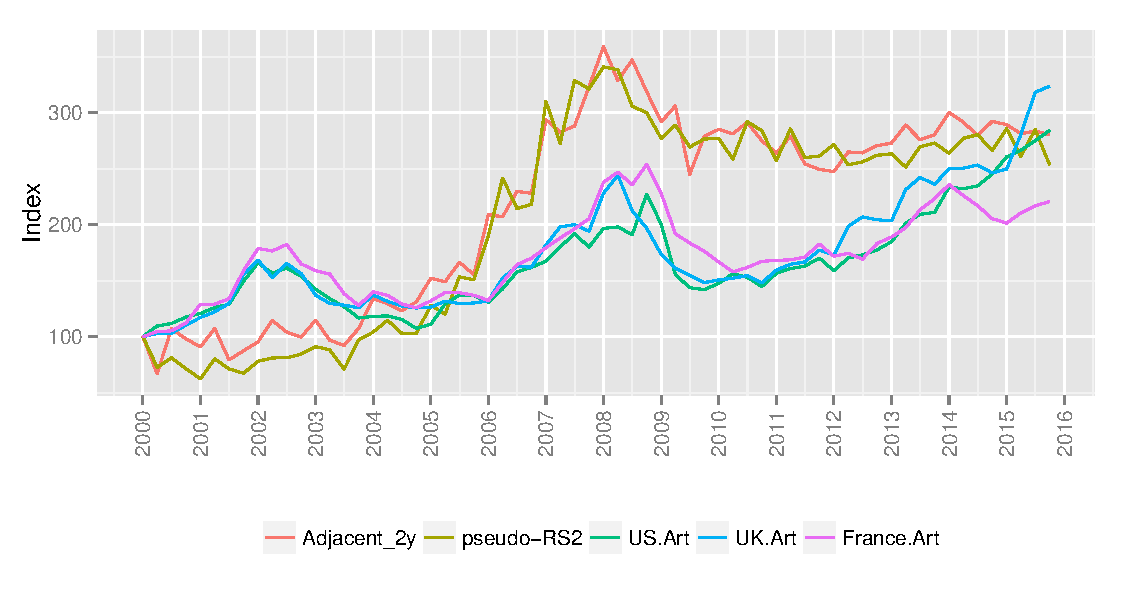
\includegraphics{Art_Price_Indices_3_files/figure-latex/figure11-1.pdf}
\caption{Comparing art price indices (2000Q1=100)}
\end{figure}

Renneboog and Spaenjers (2015) examined the extent to which art prices
generated in Western auction markets moved together since the early
1970s. Despite the cross-country variation in long-term returns, art
markets often displayed similar trends and most of the correlations in
returns were significantly positive. In this case the correlations of
returns in the South African and international art price indices,
reported in Table 4, are not significant.

Figure 12 compares the two representative art price indices with indices
for other South African assets: the JSE All Share index, the All Bond
index, and the ABSA House price index. Local asset prices have increased
much more than art prices over the entire period, which suggests that
the art price indices do not provide outlandish estimates of pure price
changes over the period. The equity and property markets also peaked at
around the same time as the art price indices. The correlations in
returns between the art price indices and the equity and property
indices, reported in Table 4, are positive and significant, although the
coefficients were relatively low. After declining for the first few
years of the sample, the art price indices experienced more rapid price
appreciation between 2005 and 2008 than the other assets.

\begin{figure}[htbp]
\centering
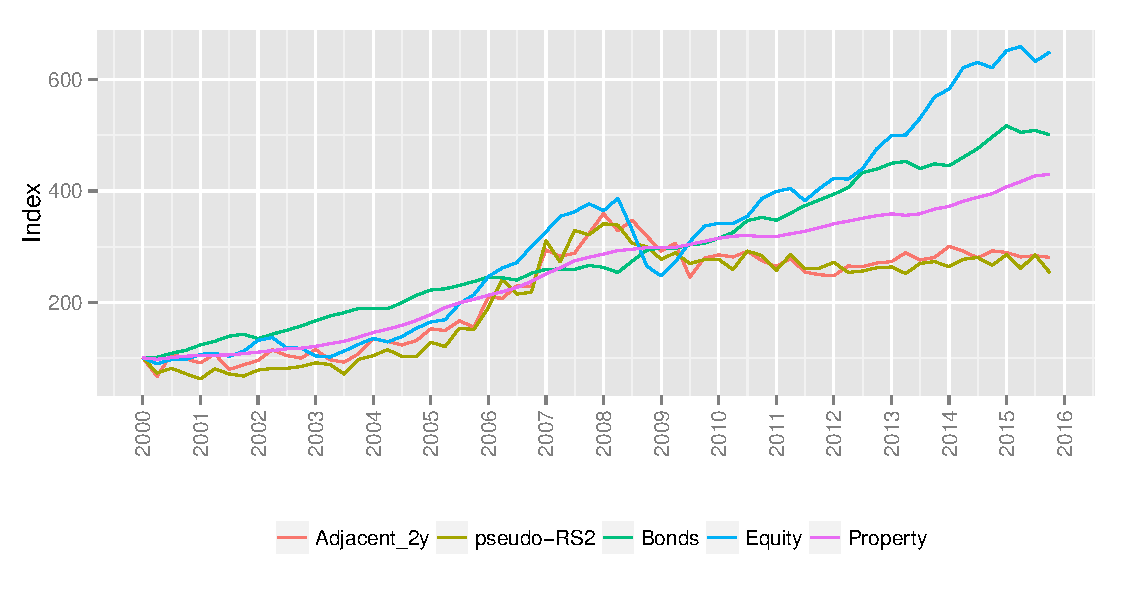
\includegraphics{Art_Price_Indices_3_files/figure-latex/figure12-1.pdf}
\caption{Comparing South African asset price indices (2000Q1=100)}
\end{figure}

\begin{table}[ht]
\centering
\caption{Correlations of returns (dlogs)} 
\scalebox{0.9}{
\begin{tabular}{rlllllll}
  \hline
 & Adj2y &  ps.RS2 & US.Art & UK.Art & French.Art & SA.Bonds & SA.Equity \\ 
  \hline
Adj2y &  &  &  &  &  &  &  \\ 
   ps.RS2 &  0.62*** &  &  &  &  &  &  \\ 
  US.Art & -0.04  & -0.07  &  &  &  &  &  \\ 
  UK.Art &  0.05  &  0.04  &  0.61*** &  &  &  &  \\ 
  French.Art &  0.04  &  0.01  &  0.72*** &  0.66*** &  &  &  \\ 
  SA.Bonds &  0.04  & -0.01  & -0.22  & -0.40**  & -0.28*  &  &  \\ 
  SA.Equity &  0.35**  &  0.33**  & -0.16  &  0.18  &  0.02  & -0.25  &  \\ 
  SA.Property &  0.39**  &  0.43*** &  0.04  &  0.06  &  0.06  &  0.05  &  0.35**  \\ 
   \hline
\end{tabular}
}
\end{table}

\subsection{Summary and Conclusion}\label{summary-and-conclusion}

This section has evaluated and compared the art price indices produced
according to central tendency, hedonic and hybrid repeat sales methods.
The regression-based indices are significantly different from the
central tendency measures and seem to produce better estimates of pure
price changes. This is confirmed by the smoothness metrics and the
consistent cyclical pattern displayed by the regression-based indices.
This shows that regression-based methods are useful in producing
quality-adjusted price indices for unique items.

Each of the regression-based methods employed above has strengths and
weaknesses. The hedonic method may suffer from omitted variable bias,
which would bias the indices, while the pseudo-repeat sales method may
control for some of this omitted variable bias, but suffer more from
possible sample selection bias. However, the regression-based indices
seem to point to the same general movement in South African art prices,
with a clear cyclical trend and a large increase in the run-up to the
Great Recession. This increase was similar to international art price
indices and traditional South African assets. The relatively consistent
picture offers some confidence that the indices provide a relatively
accurate measure of the price movements in the South African art market.

The large increase in art prices between 2005 and 2008 does not seem to
be due to a fundamental shift in the types of artworks that were sold
over that period. For instance, the top 100 artists in terms of volumes
sold, which accounts for 60\% of the volume traded and 90\% of total
turnover, has remained remarkably stable over time. Even if the exact
same artworks were not being resold, the same artists' work still made
up the vast majority of the market, and the hedonic model controls for
the different artists. It is unlikely that the results are driven by
sales of systematically better or higher quality artworks by specific
artists that appreciated in price over that period, and by sales of
systematically lower quality artworks by those artists after the crisis.
Moreover, paintings are not sold at auction only to profit from price
appreciation or capital gains. A substantial portion of consignments
come from the so-called three D's: Debt, Divorce and Death. In other
words, many sellers are forced to sell their artworks, even if those
artworks have not experienced the largest price appreciation.

In the following section the indices will be used to ascertain whether
there is evidence for the presence of a bubble in the market over this
period. In answering this question, the paper turns to literature on the
bubble detection. The bubble detection tests proposed by Phillips, Wu
and Yu (2011) are applied to the indices to investigate whether South
African art prices exhibited mildly explosive behaviour over the period.

\section{Bubble Detection}\label{bubble-detection}

Record prices for South African artworks at local and international
auctions, especially between 2008 and 2011, prompted many commentators
at the time to claim that the market was overheating and suggest the
possibility of a ``bubble'' in the market (e.g. Rabe (2011); Hundt
(2010); Curnow (2010)). According to the indices generated above there
was a substantial increase in South African art prices in the run-up to
the Great Recession. This section uses the art price indices to
investigate whether art prices exhibited bubble-like behaviour over the
sample period.

Both advanced and emerging economies experienced severe financial crises
around 2008. Yiu, Yu and Jin (2013) argued that these crises were
triggered by the collapse of bubbles in asset prices. The adverse
effects of bubbles and their related crises have led to a large
literature on financial crises and the detection of bubbles in asset
prices, including the seminal work by Kindleberger and Aliber (2005) and
the modelling approach by Phillips, Wu and Yu (2011).

The starting point is the definition of the term ``bubble''. Stiglitz
(1990) provided the following popular definition: ``\emph{{[}I{]}f the
reason the price is high today is only because investors believe that
the selling price will be high tomorrow - when `fundamental' factors do
not seem to justify such a price - then a bubble exists. At least in the
short run, the high price of the asset is merited, because it yields a
return (capital gain plus dividend) equal to that on alternative
assets.}''

According to Case and Shiller (2003), the term refers ``\emph{to a
situation in which excessive public expectations of future price
increases cause prices to be temporarily elevated.}'' According to the
New Palgrave Dictionary of Economics, ``\emph{bubbles refer to asset
prices that exceed an asset's fundamental value because current owners
believe they can resell the asset at an even higher price}''
(Brunnermeier, 2008). These definitions imply that the main features of
a bubble are that prices increase beyond what is consistent with
underlying fundamentals, and that buyers expect excessive future price
increases. In other words, a bubble consists of a sharp rise in a given
asset price, above a level sustainable by some fundamental values,
followed by a sudden collapse (Kräussl, Lehnert and Martelin, 2016).

When it comes to the art market, however, it is particularly challenging
to determine the fundamental value from which prices potentially
deviate. In the case of stocks, dividends have been used to obtain the
expected cash flow as a measure of fundamental value. Rents and
convenience yields can potentially be used for real estate prices and
commodity prices (Penasse and Renneboog, 2014).

In contrast, artworks do not generate a future income stream
(e.g.~dividends or rents) that can be discounted to determine the
fundamental value. Artworks usually have little inherent value, unless
the materials used have a high intrinsic value (Spaenjers, Goetzmann and
Mamonova, 2015). Instead, artworks are acquired for a kind of
non-monetary utility or aesthetic dividend, sometimes described as
``aesthetic pleasure'' (Gérard-Varet, 1995). This dividend can be seen
as the rent one would be willing to pay to own the artwork over a given
period. It can reflect aesthetic pleasure, but may also provide
additional utility as the signal of wealth (Mandel, 2009). The price of
an artwork should equal the present value of these future private
utility dividends over the holding period, plus the expected resale
value. The value of this dividend is unobservable and is likely to vary
tremendously across collectors, based on their motivations and
characteristics (Penasse and Renneboog, 2014). Thus, it almost
impossible to clearly determine the fundamental value of art (Kräussl,
Lehnert and Martelin, 2016).

To overcome this issue, this section follows Kräussl, Lehnert and
Martelin (2016) in using a direct method of bubble detection developed
by Phillips, Wu and Yu (2011). The approach is based on a right-tailed
augmented Dickey-Fuller (ADF) test, which can detect explosive behaviour
directly in time series. Phillips, Wu and Yu (2011) originally applied
the method to stock prices. They showed that there was evidence of
explosiveness in stock prices, but not dividend yields, implying that
price explosiveness could not be explained by developments in
fundamentals.

Since then various studies have used the method to investigate bubbles
in a number of asset markets, including real estate, commodities and
art. Jiang, Phillips and Yu (2014) employed the method to detect
explosive periods in real estate prices in Singapore. The results
suggested the existence of an explosive period from 2006Q4 to 2008Q1.
Balcilar, Katzke and Gupta (2015) used the method to date-stamp periods
of US housing price explosiveness for the period 1830-2013 and found
evidence of several bubble periods. Areal, Balcombe and Rapsomanikis
(2013) used the methodology to test for the presence of periods of
explosive prices in agricultural markets and found that bubbles occurred
for certain commodities, especially around 2007 and 2008.
Figuerola-Ferretti, Gilbert and Mccrorie (2015) applied the method to
examine the recent behaviour of non-ferrous metals futures prices on the
London Metal Exchange. They found that certain commodity futures markets
were prone to bubble-like phenomena and that the majority of the bubbles
occurred between August 2007 and July 2008.

In the context of art, Kräussl, Lehnert and Martelin (2016) used the
method to detect explosive behaviour in the prices of four different art
market segments (\emph{Impressionist and Modern}, \emph{Post-war and
Contemporary}, \emph{American} and \emph{Latin American}). They found
evidence of explosive behaviour in prices and identified historical
bubble episodes in the ``\emph{Post-war and Contemporary}'' and
``\emph{American}'' art market segments, around 2006-2008 and 2005-2008
respectively. The following section sets out the bubble detection
framework used to test for the presence of bubble-like behaviour in
South African art prices over the period.

\subsection{Bubble Detection
Framework}\label{bubble-detection-framework}

The most commonly used detection methods are based on the present value
model and the rational bubble assumption. According to the present value
model, under rational expectations, the price of an asset is equal to
the present value of its future income stream, i.e.~the expected
fundamental value: \[P_t = \frac{1}{1+r_f} E_t(P_{t+1} + \gamma_{t+1})\]
where \(r_f\) is the constant discount rate, \(P_t\) is the asset price
at time \(t\), and \(\gamma_{t+1}\) is the payment received
(e.g.~dividends, rents or a convenience yield) for owning the asset
between \(t\) and \(t+1\). When \(t+n\) is far into the future,
\(\frac{1}{1+r_f} E_t(P_{t+n})\) does not affect \(P_t\), as it tends to
zero as \(n\) becomes infinitely large. The present value or market
fundamental solution could be written as:
\[F_t = E_t[\sum_{i=1}^n \frac{1}{1+r_f} (\gamma_{t+n})]\]

Rational bubbles arise when investors are willing to pay more than the
fundamental value to buy an asset because they expect the asset price to
significantly exceed its fundamental value in the future. When rational
bubbles are present, the asset price is composed of the fundamental
component and a bubble component (Yiu, Yu and Jin, 2013). In other
words, if a gap between the market fundamental solution and the actual
price exists and the terminal condition does not hold, an additional
``bubble component'', \(B_t\), has to be added to the solution of
equation: \(P_t = F_t + B_t\). In this case \(F_t\) is called the
fundamental component of the price and \(B_t\) is any random variable
that satisfies the following condition:
\[B_t = \frac{1}{1+r_f} E_t(B_{t+n})\]

Thus, the bubble component is included in the price process, and
anticipated to be present in the next period with an expected value of
\((1 + r_f)\) multiplied by its current value. Being in line with the
rational expectations framework, the bubble component is called a
``rational bubble'' (Kräussl, Lehnert and Martelin, 2016).

The statistical properties of \(P_t\) are determined by those of \(F_t\)
and \(B_t\). In the absence of a bubble, when \(B_t=0\), the degree of
non-stationarity in \(P_t\) is controlled by the nature of the series
\(F_t\), which in turn is determined by the properties of \(\gamma_t\).
The current price of the commodity is therefore determined by market
fundamentals: for example, if \(\gamma_t\) is an I(1) process then
\(P_t\) would be an I(1) process.

When a bubble is present, if \(B_t \neq 0\), current prices \(P_t\) will
exhibit explosive behaviour, as \(B_t\) reflects a stochastic process in
which the expected value of next period's value, forecast on the basis
of the current period's information, is greater than or equal to the
current period's value (Kräussl, Lehnert and Martelin, 2016). In the
absence a structural change in the fundamental process or explosiveness
in the fundamentals, a period of explosive prices must have a
non-fundamental explanation. Under the assumed properties of
\(\gamma_t\), the observation of mildly explosive behaviour in \(P_t\)
(i.e.~non-stationarity of an order greater than unit root
non-stationarity) will offer evidence of bubble behaviour. This
expression embodies an explosive property and introduces ``bubble''
movements in the price over the fundamental component (Areal, Balcombe
and Rapsomanikis, 2013). Thus, the theory predicts that if a bubble
exists, prices should inherit its explosiveness property. This enables
the formulation of statistical tests that try to detect evidence of
explosiveness in the data (Caspi, 2013).

Given the different stochastic properties of the fundamental and bubble
components, early tests were based on unit root and cointegration tests.
Campbell and Shiller (1987) suggested a unit root test for explosiveness
in prices, based on the idea that the gap between the asset price and
the fundamental value will exhibit explosive behaviour during the
process of bubble formation. They identified two scenarios that strongly
suggest the presence of a rational bubble. In the first case, the asset
price is non-stationary while the fundamental value is stationary. In
the second, the asset price and fundamental value are both
non-stationary (Yiu, Yu and Jin, 2013). In this case, if the asset price
and its fundamental value are co-integrated, their non-stationary
behaviour does not provide evidence of a bubble. Diba and Grossman
(1988) showed that if fundamental values are not explosive, the
explosive behaviour in prices is a sufficient condition for the presence
of bubble.

However, unit root and cointegration tests are not capable of detecting
explosive prices when a series contains periodically collapsing bubbles.
Evans (1991) argued that explosive behaviour is only temporary in the
sense that bubbles eventually collapse and that asset prices may appear
more like I(1) or even stationary series than an explosive series,
thereby confounding empirical evidence. Using simulated data Evans
(1991) showed that these tests could not differentiate between a
periodically collapsing bubble and a stationary process. A series
containing periodically collapsing bubbles could therefore be
interpreted by the standard unit root tests as a stationary series,
leading to the incorrect conclusion that the data contained no explosive
behaviour (Phillips, Wu and Yu, 2011).

A number of methods have been proposed to deal with this critique (Yiu,
Yu and Jin, 2013). The recursive tests proposed by Phillips, Wu and Yu
(2011) and Phillips, Shi and Yu (2012) are not subject to this criticism
and can effectively distinguish unit root processes from periodically
collapsing bubbles, as well as date-stamp their origin and collapse. The
tests proposed by Phillips, Wu and Yu (2011) are based on the idea of
repeatedly implementing a right-tailed unit root test. The method
involves the estimation of an autoregressive model, starting with a
minimum fraction of the sample and incrementally expanding the sample
forward.

The model typically takes the following form:
\[\Delta y_t = \alpha_w + (\delta_w - 1) y_{t-1} + \sum_{i=1}^k \phi_w^i \Delta y_{t-i} + \epsilon_t\]
where \(y_t\) is the asset price series, \(\alpha\), \(\delta\) and
\(\phi\) are the parameters to be estimated, \(w\) is the sample window
size, \(k\) is the lag order, and \(\epsilon_t\) is the white noise
error term.

A sample of Augmented Dickey-Fuller test statistics are calculated from
each regression. The null hypothesis of a unit root \((\delta = 1)\) is
tested against the right-tailed alternative of mildly explosive
behaviour \((\delta > 1)\). The supremum value of the ADF sequence is
then used to test for mildly explosive behaviour. By looking directly
for evidence of explosive behaviour, the test avoids the risk of
misinterpreting a rejection of the null hypothesis due to stationary
behaviour.

The method also allows date-stamping of the origination and termination
dates by matching the time series of the recursive test statistics to
the critical value sequence. In other words, each element of the
estimated ADF sequence is compared to the corresponding right-tailed
critical values of the ADF statistic to identify a bubble period. The
estimated origination point of a bubble is the first observation in
which ADF value crosses the corresponding critical value (from below),
while the estimated termination point is the first observation
thereafter when the ADF value crosses below the critical value (Caspi,
2013).

A limitation of the method is that it is designed to analyse a single
bubble episode. Phillips, Shi and Yu (2012) expanded the method to
account for the possibility of multiple bubbles. The sample is extended
by varying both the starting and ending points of the sample over a
feasible range of windows. The moving window provides greater
flexibility in choosing a subsample that contains a bubble (Yiu, Yu and
Jin, 2013). Thus, the method of Phillips, Wu and Yu (2011) is consistent
and particularly effective when there is a single explosive episode in
the data, while the method of Phillips, Shi and Yu (2012) can identify
multiple explosive episodes. Simulations by Homm and Breitung (2012)
indicated that the procedure worked satisfactorily against other time
series tests for the detection of bubbles and was particularly effective
for real-time bubble detection.

\subsection{Bubble Detection Results}\label{bubble-detection-results}

This section tests whether the South African art market has exhibited
bubble-like behaviour over the sample period, focusing on a specific
aspect of bubbles: explosive prices. This section follows the convention
of using the log value of real asset prices, deflated with the CPI (e.g.
Kräussl, Lehnert and Martelin (2016), Caspi (2013) and Balcilar, Katzke
and Gupta (2015)). In this case there is only one potential bubble
episode, so the Phillips, Wu and Yu (2011) method should be sufficient
to provide consistent evidence of mildly explosive behaviour.

As explained above, the method involves the estimation of an
autoregressive model, starting with a minimum fraction of the sample and
incrementally expanding the sample forward. The model starts with 3
years (i.e.~12 observations) and expands the sample by one observation
each time. Each estimation yields an ADF statistic. In this case, there
does not seem to be a deterministic drift present in the log real art
price indices and the intercept is not statistically significant at
conventional levels. However, as the results might be sensitive to model
formulation, two versions of the autoregression models are used: one
without a constant or trend and one with a constant or drift term. Lags
are included to take possible autocorrelation of the residuals into
account and the number of lags \(k\) is chosen with the Akaike
Information Criterion.

Critical values for the tests are derived from Monte Carlo simulations
of a random walk process, both including and excluding a drift term,
with 2000 replications. In their original study Phillips, Wu and Yu
(2011) use a random walk without drift to estimate the null hypothesis.
According to Phillips, Shi and Yu (2014), when the model is estimated
with a non-zero drift it produces a dominating deterministic component
that has an empirically unrealistic explosive form. They argue that
these forms are unreasonable for most economic and financial time series
and an empirically more realistic description of explosive behaviour is
given by models formulated without a constant or deterministic trend.
Nevertheless, as a robustness check the models were formulated with and
without a constant or drift term included.\footnote{Phillips, Shi and Yu
  (2014) suggested a random walk process with an asymptotically
  negligible drift might be useful for allowing for intermediate cases
  between a model with no drift and one with a drift term included,
  i.e.~cases where there may be drift in the data but it may not be the
  dominant component. Such a model may take the following form:
  \(y_t = d T^{-\eta} + \theta y_{t-1} + \epsilon_t\), where \(d\),
  \(\eta\) and \(\theta\) are constant, \(T\) is the sample size, and
  \(\epsilon_t\) is the white noise error term. The deterministic
  component depends on the sample size T and the localising parameter
  \(\eta\). When \(\eta > 0\) the drift term is small relative to the
  linear trend. The null model becomes a model without drift when
  \(\eta \to \infty\) and a model with drift when \(\eta \to 0\). The
  results may be sensitive to the value of \(\eta\), so they recommend
  reporting the results for a range of values of \(\eta\). In this case,
  different values of \(\eta\) produce qualitatively similar results.}

The supremum ADF test statistics from to both formulations are above the
95\% critical values for each of the indices, except for the median
index. Therefore, the null hypothesis of a unit root may be rejected in
favour of the alternative hypothesis for each of the indices, except the
median index. This provides evidence that real art prices experienced
periods of explosiveness over the sample.

The method can now be used to date stamp potential bubble periods.
Figure 13 and Figure 14 illustrate the date stamping procedure for three
representative series: median values, the 2-year adjacent period hedonic
index and the second version (larger sample) of the ps-RS index. Figure
13 illustrates the case of no drift term, while Figure 14 illustrates
the case with a drift term. The figures compare the ADF test static
sequence to the 95\% and 99\% critical value sequences. In both cases
the test statistic sequences breach the 95\% critical values in the
run-up to the financial crisis (2005 and 2006 respectively), before
falling below the critical values. The sequence of test statistics for
the ps-RS index is higher than for the full sample hedonic index, and
breaches the 99\% critical value.

\begin{figure}[htbp]
\centering
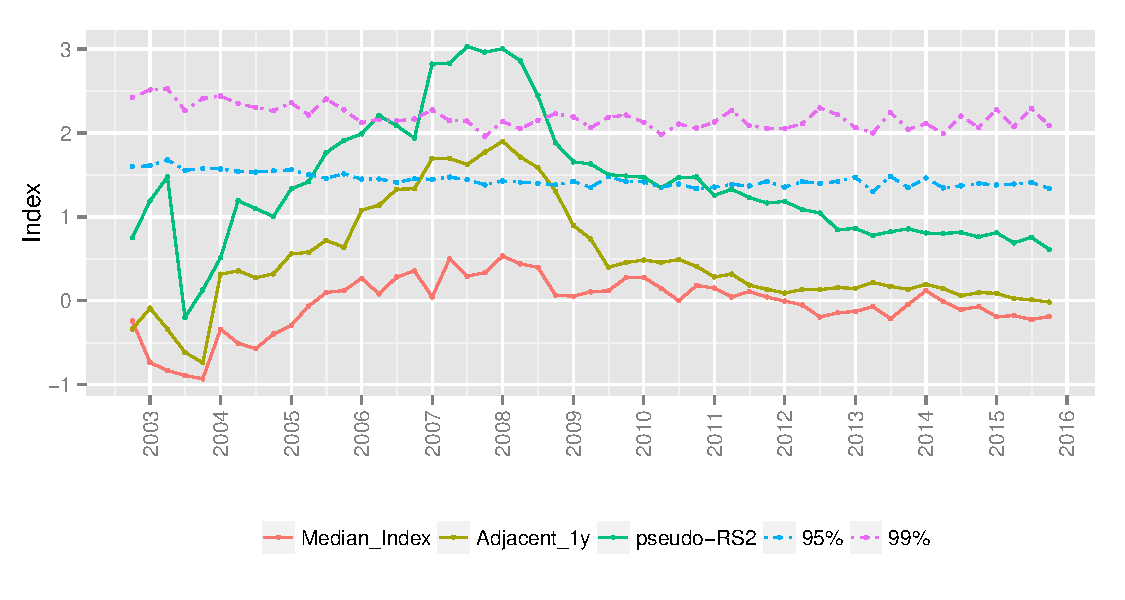
\includegraphics{Art_Price_Indices_3_files/figure-latex/figure13-1.pdf}
\caption{Test statistics and critical values for models without drift}
\end{figure}

\begin{figure}[htbp]
\centering
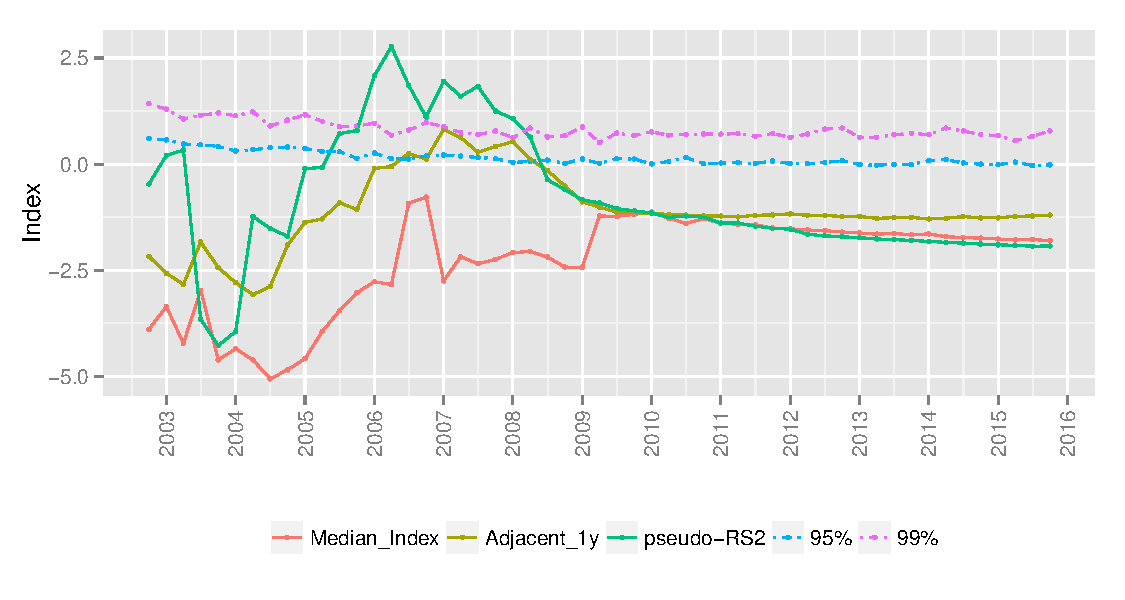
\includegraphics{Art_Price_Indices_3_files/figure-latex/figure14-1.pdf}
\caption{Test statistics and critical values for models with drift}
\end{figure}

Table 5 reports the origination and termination dates for all of the
periods of explosive behaviour, based on 95\% critical values. The test
statistic sequences for the hedonic indices all indicate a period of
explosive prices beginning around 2006/2007 and ending in 2008. The test
statistics for the ps-RS indices indicate periods of explosive behaviour
that were slightly longer, beginning around 2005/2006 and ending in 2008
or even 2010, depending on the specification. The preferred method in
terms of index smoothness (i.e.~the ps-RS2 index) therefore suggests a
slightly longer period of bubble formation. Phillips, Shi and Yu (2012)
recommend that only explosive periods lasting more than log(T) units of
time should be identified as bubble periods. In this case this implies
that the bubble should be at least 4 quarters in length and virtually
all of the explosive periods identified satisfy this requirement.

\begin{table}[ht]
\centering
\caption{Dates of explosive behaviour} 
\begin{tabular}{rllll}
  \hline
 & None-Start & None-End & Drift-Start & Drift-End \\ 
  \hline
Fisher\_Index & 2008 Q1 & 2010 Q3 & 2008 Q1 & 2009 Q2 \\ 
  Hedonic\_full & 2007 Q1 & 2008 Q3 & 2007 Q1 & 2008 Q2 \\ 
  Adjacent\_1y & 2007 Q1 & 2008 Q3 & 2006 Q3 & 2008 Q2 \\ 
  Adjacent\_2y & 2007 Q1 & 2008 Q4 & 2006 Q3 & 2008 Q2 \\ 
  Rolling & 2007 Q4 & 2008 Q3 & 2007 Q1 & 2008 Q2 \\ 
  pseudo-RS1 & 2005 Q3 & 2010 Q1 & 2006 Q1 & 2008 Q2 \\ 
  pseudo-RS2 & 2005 Q3 & 2010 Q4 & 2005 Q3 & 2008 Q2 \\ 
   \hline
\end{tabular}
\end{table}

The dates identified correspond with many of the explosive periods
identified in the literature for a range of assets. In the context of
art, Kräussl, Lehnert and Martelin (2016) identified bubble periods for
the ``\emph{Post-war and Contemporary}'' art segment between 2006 and
2008 and for the ``\emph{American}'' art segments between 2005 and 2008,
which also corresponds to the pre-financial crisis period.
Interestingly, their data pointed to evidence in the formation of
another bubble in these market segments around the start of 2011. This
is not present in the South African art market, which has remained
relatively flat since 2010.

It is also interesting that many of the headline grabbing auction
records for the South African art market occurred in 2011, well after
the period of explosive behaviour. This corresponds to findings by
Spaenjers, Goetzmann and Mamonova (2015), who observed that the timing
of record prices does not always coincide with periods of general price
increases. They argue that auction price records are often set in
situations characterised by extreme supply constraints, social
competition among ``nouveaux riches'', resolution of uncertainty about
the potential resale value, and idiosyncratic shifts in hedonic weights.

\subsection{Discussion}\label{discussion}

This section has applied the reduced-form bubble detection method
developed by Phillips, Wu and Yu (2011) to test for periods of explosive
behaviour in the art price indices. The use of recursive tests enables
the identification of mildly explosive subsamples in the series. The
results indicate that there is evidence of bubble-like behaviour in all
of the regression-based art price indices, whereas the simple median
index does not exhibit such behaviour. Again, this implies that it is
important to control for the composition or quality-mix of sales when
estimating indices for unique items. The regression-based indices
provide relatively consistent results in terms of the explosive periods
in the South African art market, with a potential bubble most likely
beginning in 2006 and ending in 2008.

The results implicitly assume that the aesthetic or utility dividends
associated with South African art did not exhibit explosive behaviour
over the period. Aesthetic dividends fluctuate over time as they depend
on buyers' willingness to pay for art, which in turn depends on
preferences and wealth. However, preferences regarding art and culture
would have had to fluctuate dramatically to explain the movements in art
prices over the period. Even if trends can temporarily emerge for
specific artists or schools of art, previous findings in the literature
have shown that preferences tend to be very stable, even in the long run
(Penasse and Renneboog, 2014). The aesthetic dividend can also fluctuate
as wealth fluctuates over time (Spaenjers, Goetzmann and Mamonova,
2015). The literature has provided evidence supporting this idea, with
Goetzmann, Renneboog and Spaenjers (2011) finding cointegrating
relationships between top incomes and art prices. However, it is
unlikely that aesthetic dividends, or factors such as collectors'
preferences and wealth, experienced similar explosive behaviour over the
period.

Although the method provides a consistent basis for identifying periods
of explosive behaviour, it does not provide an explanation of the bubble
episode. The findings are compatible with several different
explanations, including rational bubbles, herd behaviour, and rational
responses to fundamentals (Phillips, Wu and Yu, 2011).

The periods of explosive prices could be compatible with a rational
bubble, where investors are willing to pay more than their private value
for an artwork, because they expect to resell later at a higher price.
Gérard-Varet (1995) argued that the sharp rise in world art prices in
the late 1980s could be explained by a rational bubble, where investors
believed that although prices had attained unsustainable levels the
short run, prospects for continued gains were sufficient to compensate
for the risk that the bubble might burst. Prices increase at an
accelerating rate because the probability of a crash increases and
rational investors require an increasing risk premium to cover this
higher probability of a crash (Rosser, Rosser and Gallegati, 2012).

Investors might think that an artwork that they would normally consider
too expensive is now an acceptable purchase because they will be
compensated by further price increases. During a bubble investors may
also worry that if they do not buy now, they will not be able to afford
the artwork later. The expectation of large price increases may have a
strong impact on demand if investors think that prices are unlikely to
fall, or not likely to fall for long, so that there is little perceived
risk associated with a purchase (Case and Shiller, 2003).

Penasse and Renneboog (2014) argue that limits to arbitrage induce a
speculative component to art prices. High transaction costs and
short-selling constraints could lead to prices diverging from
fundamental levels, as they prevent arbitrageurs from pulling back
prices to fundamentals (Balcilar, Katzke and Gupta, 2015). When prices
are high, pessimists would like to short sell, but instead simply stay
out of the market or sell to optimists at inflated prices. Optimists may
be willing to pay higher prices than their own valuations, because they
expect to resell to even more optimistic investors in the future. The
difference between their willingness to pay and their own optimistic
valuation is the price of the option to resell the asset in the future.
The price of the resale option imparts a bubble component in asset
prices, and can explain price fluctuations unrelated to fundamentals.
These market failures hamper the ability of markets to correct price
inefficiencies and implies that periods of bubble-like behaviour could
exist with relatively little scope for arbitrage. This is especially
applicable to art markets, where transaction costs are high, short
selling is not possible, and without a rental market the only
possibility to make a profit is by reselling at a higher price (Penasse
and Renneboog, 2014).

Penasse and Renneboog (2014) investigated this theory by looking at the
behaviour of art prices and volumes. They found that the art market was
subject to frequent booms and busts in both prices and volumes. They
showed that booms in volume were mainly driven by short-term
transactions, which were interpreted as speculative transactions or
trading frenzies. Given the high transaction costs that characterise the
art market, it is unlikely that these artworks were purchased for the
pure aesthetic dividends. The positive correlation between prices and
volumes was persistent across art movements, and was larger for the most
volatile segments of the art market (i.e.~Modern and Contemporary art).
When trading volume was high, they found that buyers tended to overpay,
in that high volume predicted negative returns in subsequent years. This
provides evidence for resale option theory and speculative trading
models of bubble formation, which predict that speculative trading can
generate significant price bubbles, even if trading costs are large and
leverage impossible.

Balcilar, Katzke and Gupta (2015) argued that large price increases in
the short term could lead to higher allocation towards assets
experiencing high capital growth. This, in turn, feeds into more demand
and even higher prices, potentially driving an episode of unsustainable
asset price increases, particularly as a result of factors inherent to
art purchases, such as high transaction costs and difficulties with
short-selling. Similarly, Mandel (2009) analysed the satisfaction
derived from conspicuous consumption, which increases as the value of
art increases. The part of the aesthetic dividend that is a signal of
wealth could plausibly lead to price increases, which in turn could lead
to another increase in the dividend related social status consumption.

In general, speculative bubbles can act like self-fulfilling prophecies.
Prices increase because agents expect them to do so, with this ongoing
expectation providing the increasing demand that keeps prices rising. If
prices stop rising due to some exogenous shock like the financial
crisis, this breaks the expectation and the speculative demand suddenly
disappears, sending prices back towards their fundamental value, where
there is no expectation of the price rising (Rosser, Rosser and
Gallegati, 2012).

Kindleberger and Aliber (2005) argued that a boom in one market often
spills over into other markets. A famous example in the context of art
is the link between the boom in Japanese stock and real estate prices
and the Impressionist art market in the second half of the 1980s. Hiraki
\emph{et al.} (2009) found a strong correlation between Japanese stock
prices and the demand for art by Japanese collectors, leading to an
increase in the price of Impressionist art during this period. Kräussl,
Lehnert and Martelin (2016) found corroborating evidence of a bubble
period in the ``Impressionist and Modern'' art segment between 1986 and
1991. During this period Japanese credit was freely available, backed by
increasing values of stocks and real estate, which led to a consumption
and investment spree through the wealth effect. Japanese investors
invested heavily in international art and particularly French
Impressionist art in the late 1980s. Luxury consumption by Japanese art
collectors increased international art prices until the art bubble burst
as a direct consequence of the collapse of the Japanese real estate
market (Penasse and Renneboog, 2014).

Similarly, the run-up to the financial crisis saw large increases in
asset prices and credit expansion. It is likely that these conditions
contributed to the explosive behaviour in South African art prices
between 2006 and 2008. The financial crisis caused the bubble to burst
and led to a decline in South African art prices. While an in depth
investigation is outside the scope of the paper, it does illustrate the
usefulness of the art price indices to investigate developments in the
South African art market.

\section{Conclusion}\label{conclusion}

To date there has been little research on the South African art market
and particularly trends in art prices. This paper has attempted to make
three contributions to the literature. The first was to estimate new
price indices for the South African art market since the turn of the
millennium. Three broad methodologies were used to estimate
quality-adjusted price indices for South African art: central tendency,
hedonic and hybrid repeat sales methods.

Each of the methods has strengths and weaknesses. The hedonic regression
method is able to control more adequately for quality-mix changes than
central tendency methods. The main shortcoming of the hedonic method is
that it has potential omitted variable bias, which might bias the
coefficients and therefore the indices. The second contribution was to
apply a simple hybrid repeat sales method, which has not been attempted
for art prices in any country. This approach addressed the problem of
lack of repeat sales observations in the sample and to some extent the
potential omitted variable bias inherent in the hedonic method, although
it may suffer from potential sample selection bias.

The regression-based indices were significantly different from the
central tendency measures. They seemed to produce better estimates of
pure price changes, as shown by the smoothness metrics. This
demonstrates the importance of regression-based methods to produce
quality-adjusted price indices for unique assets. The regression-based
indices seem to point to the same general movement in South African art
prices, with a clear cyclical trend and a large increase in the run-up
to the Great Recession. This increase was similar to international art
price indices and traditional South African assets. The relatively
consistent picture offers some confidence that the indices provide a
relatively accurate measure of the general price movements in the South
African art market.

The third contribution was to the use the art price indices to look for
mildly explosive behaviour in prices over the sample period, using a
reduced-form bubble detection method. The results indicated that there
was evidence of bubble-like behaviour in all of the regression-based art
price indices. The regression-based indices seem to point to consistent
evidence of explosive prices in the run-up to the Great Recession, with
the bubble period starting around 2006 and ending around 2008.

The art price indices are useful for investigating and understanding
developments in the South African art market. In this paper the indices
were studied for evidence of a bubble in the market. Further research
applications might consider the risk-return profile of art as an asset
class and evaluate whether art could form part of an optimal investment
portfolio. Conventional wisdom says that the top artworks by established
artists tend to outperform the rest of the market (Mei and Moses, 2002).
Another application would be to examine this so-called Masterpiece
effect by looking at different parts of the distribution of art prices.
Potential drivers or factors that influence the fluctuations in art
prices over time, such as wealth effects, might also be investigated.
The quality-adjusted art price indices can facilitate these inquiries
and enable one to be more concrete about developments in the South
African art market.

\section*{References}\label{references}
\addcontentsline{toc}{section}{References}

\hyperdef{}{ref-Anderson1974}{\label{ref-Anderson1974}}
Anderson, R. C. (1974) `Paintings as an investment', \emph{Economic
Inquiry}, 12, pp. 13--26.

\hyperdef{}{ref-Areal2013}{\label{ref-Areal2013}}
Areal, F. J., Balcombe, K. and Rapsomanikis, G. (2013) `Testing for
bubbles in agriculture commodity markets', \emph{Munich Personal RePEc
Archive}. (MPRA paper no. 48015), (48015).

\hyperdef{}{ref-Aye2014}{\label{ref-Aye2014}}
Aye, G. C., Balcilar, M., Bosch, A. and Gupta, R. (2014) `Housing and
the business cycle in South Africa', \emph{Journal of Policy Modeling}.
The Society for Policy Modeling, 36(3), pp. 471--491.
\href{http://doi.org/10.1016/j.jpolmod.2014.03.001}{doi: 10.1016/j.jpolmod.2014.03.001}.

\hyperdef{}{ref-Bailey1963a}{\label{ref-Bailey1963a}}
Bailey, M. J., Muth, R. F. and Nourse, H. O. (1963) `A regression method
for real estate price index construction', \emph{Journal of the American
Statistical Association}, 58(304), pp. 933--942.
\href{http://doi.org/10.1080/01621459.1963.10480679}{doi: 10.1080/01621459.1963.10480679}.

\hyperdef{}{ref-Balcilar2015}{\label{ref-Balcilar2015}}
Balcilar, M., Katzke, N. and Gupta, R. (2015) `Identifying Periods of US
Housing Market Explosivity', \emph{University of Pretoria: Department of
Economics Working Paper Series}, 2015-44.

\hyperdef{}{ref-Botha2016}{\label{ref-Botha2016}}
Botha, F., Snowball, J. and Scott, B. (2016) `Art investment in South
Africa: Portfolio diversification and art market efficiency',
\emph{South African Journal of Economic and Management Sciences}, 19(3),
pp. 358--368.

\hyperdef{}{ref-Brunnermeier2008}{\label{ref-Brunnermeier2008}}
Brunnermeier, M. K. (2008) `Bubbles', in Durlauf, S. N. and Blume, L. E.
(eds) \emph{New palgrave dictionary of economics}. 2nd edn. Palgrave
Macmillan (i), pp. 1--17.

\hyperdef{}{ref-Calomiris2016}{\label{ref-Calomiris2016}}
Calomiris, B. C. W. and Pritchett, J. (2016) `Betting on Secession:
Quantifying Political Events Surrounding Slavery and the Civil War',
\emph{American Economic Review}, 106(1), pp. 1--23.

\hyperdef{}{ref-Campbell1987}{\label{ref-Campbell1987}}
Campbell, J. Y. and Shiller, R. J. (1987) `Cointegration and Tests of
Present Value Models', \emph{The Journal of Political Economy}, 95(5),
pp. 1062--1088.
\href{http://doi.org/10.1086/261502}{doi: 10.1086/261502}.

\hyperdef{}{ref-Campbell2009}{\label{ref-Campbell2009}}
Campbell, R. J. (2009) `Art as a Financial Investment',
\emph{Collectible Investments for the High Net Worth Investor}, pp.
119--150.
\href{http://doi.org/10.1016/B978-0-12-374522-4.00006-8}{doi: 10.1016/B978-0-12-374522-4.00006-8}.

\hyperdef{}{ref-Capgemini2010}{\label{ref-Capgemini2010}}
Capgemini (2010) \emph{World Wealth Report 2010}. Capgemini \& Merrill
Lynch Global Wealth Management.

\hyperdef{}{ref-Capgemini2013}{\label{ref-Capgemini2013}}
Capgemini (2013) \emph{World Wealth Report 2013}. Capgemini \& RBC
Wealth Management.

\hyperdef{}{ref-Case1991}{\label{ref-Case1991}}
Case, B. and Quigley, J. M. (1991) `The Dynamics of Real Estate Prices',
\emph{The Review of Economics and Statistics}, 73(1), pp. 50--58.

\hyperdef{}{ref-Case1987}{\label{ref-Case1987}}
Case, K. E. and Shiller, R. J. (1987) `Prices of single-family homes
since 1970: new indexes for four cities', \emph{New England Economic
Review}, (September), pp. 45--56.
\href{http://doi.org/10.3386/w2393}{doi: 10.3386/w2393}.

\hyperdef{}{ref-Case2003}{\label{ref-Case2003}}
Case, K. E. and Shiller, R. J. (2003) `Is There a Bubble in the Housing
Market?', \emph{Brookings Papers on Economic Activity}, 34(2), pp.
299--362.

\hyperdef{}{ref-Caspi2013}{\label{ref-Caspi2013}}
Caspi, I. (2013) `Rtadf: Testing for Bubbles with EViews', \emph{Munich
Personal RePEc Archive}, (58791).

\hyperdef{}{ref-Collins2009}{\label{ref-Collins2009}}
Collins, A., Scorcu, A. and Zanola, R. (2009) `Reconsidering hedonic art
price indexes', \emph{Economics Letters}. Elsevier B.V., 104(2), pp.
57--60.
\href{http://doi.org/10.1016/j.econlet.2009.03.025}{doi: 10.1016/j.econlet.2009.03.025}.

\hyperdef{}{ref-Curnow2010}{\label{ref-Curnow2010}}
Curnow, R. (2010) `South Africa's Booming Art Market', \emph{CNN World}.
Available at:
\url{http://edition.cnn.com/2010/WORLD/africa/06/17/kentridge.south.africa.art.star/}.

\hyperdef{}{ref-Deng2012}{\label{ref-Deng2012}}
Deng, Y., McMillen, D. and Sing, T. (2012) `Private Residential Price
Indices in Singapore: A Matching Approach', \emph{Regional Science and
Urban Economics}, 42(3), pp. 485--494.

\hyperdef{}{ref-Diba1988}{\label{ref-Diba1988}}
Diba, B. T. and Grossman, H. I. (1988) `The Theory of Rational Bubbles
in Stock Prices', \emph{Economic Journal}, 98(392), pp. 746--754.

\hyperdef{}{ref-Dorsey2010}{\label{ref-Dorsey2010}}
Dorsey, R. E., Hu, H., Mayer, W. J. and Wang, H. C. (2010) `Hedonic
versus repeat-sales housing price indexes for measuring the recent
boom-bust cycle', \emph{Journal of Housing Economics}. Elsevier Inc.,
19(2), pp. 87--105.
\href{http://doi.org/10.1016/j.jhe.2010.04.001}{doi: 10.1016/j.jhe.2010.04.001}.

\hyperdef{}{ref-Econex2012}{\label{ref-Econex2012}}
Econex (2012) \emph{Citadel Art Price Index}. March, pp. 1--20.

\hyperdef{}{ref-Els2010}{\label{ref-Els2010}}
Els, M. and Von Fintel, D. (2010) `Residential property prices in a
submarket of South Africa: Separating real returns from attribute
growth', \emph{South African Journal of Economics}, 78(4), pp. 418--436.
\href{http://doi.org/10.1111/j.1813-6982.2010.01244.x}{doi: 10.1111/j.1813-6982.2010.01244.x}.

\hyperdef{}{ref-Epple1987}{\label{ref-Epple1987}}
Epple, D. (1987) `Hedonic Prices and Implicit Markets: Estimating Demand
and Supply Functions for Differentiated Products', \emph{Journal of
Political Economy}, 95(1), pp. 59--80.

\hyperdef{}{ref-Eurostat2013}{\label{ref-Eurostat2013}}
Eurostat (2013) \emph{Handbook on Residential Property Price Indices
(RPPIs)}. Luxembourg: Publications Office of the European Union, 2013:
European Commission (November 2009).

\hyperdef{}{ref-Evans1991}{\label{ref-Evans1991}}
Evans, G. W. (1991) `Pitfalls in Testing for Explosive Bubbles in Asset
Prices', \emph{American Economic Review}, 81(4), pp. 922--930.
\href{http://doi.org/10.2307/2006651}{doi: 10.2307/2006651}.

\hyperdef{}{ref-Fedderke2014}{\label{ref-Fedderke2014}}
Fedderke, J. W. and Li, K. (2014) `Art in Africa: Market Structure and
Pricing Behavior in the South African Fine Art Auction Market , 2009 -
2013'. Economic Research Southern Africa (ERSA working paper 466).

\hyperdef{}{ref-Figuerola2015}{\label{ref-Figuerola2015}}
Figuerola-Ferretti, I., Gilbert, C. L. and Mccrorie, R. (2015) `Testing
for Bubbles in LME Non-Ferrous Metals Prices', \emph{Journal of Time
Series Analysis}, 36, pp. 763--782.

\hyperdef{}{ref-Findlay2012}{\label{ref-Findlay2012}}
Findlay, M. (2012) \emph{The Value of Art: Money, Power, Beauty}. 1st
Englis. Munich: Prestel Publishing.

\hyperdef{}{ref-Froeb1994}{\label{ref-Froeb1994}}
Froeb, L. and Koyak, R. (1994) `Measuring and Comparing Smoothness in
Time Series: The Production Smoothing Hypothesis', \emph{Journal of
Econometrics}, 64, pp. 97--122.

\hyperdef{}{ref-Gerard-Varet1995}{\label{ref-Gerard-Varet1995}}
Gérard-Varet, L. V. (1995) `On pricing the priceless: Comments on the
economics of the visual art market', \emph{European Economic Review},
39, pp. 509--518.

\hyperdef{}{ref-Goetzmann2011}{\label{ref-Goetzmann2011}}
Goetzmann, W., Renneboog, L. and Spaenjers, C. (2011) `Art And Money',
\emph{The American Economic Review}, 101(3), pp. 222--246.

\hyperdef{}{ref-Griliches1961}{\label{ref-Griliches1961}}
Griliches, Z. (1961) `Hedonic Price Indexes for Automobiles: An
Econometric of Quality Change', in Committee, R. of the P. S. R. (ed.)
\emph{The price statistics of the federal goverment}. NBER, pp.
173--196.
\href{http://doi.org/10.1017/CBO9781107415324.004}{doi: 10.1017/CBO9781107415324.004}.

\hyperdef{}{ref-Guo2014}{\label{ref-Guo2014}}
Guo, X., Zheng, S., Geltner, D. and Liu, H. (2014) `A new approach for
constructing home price indices: The pseudo repeat sales model and its
application in China', \emph{Journal of Housing Economics}. Elsevier
Inc., 25, pp. 20--38.
\href{http://doi.org/10.1016/j.jhe.2014.01.005}{doi: 10.1016/j.jhe.2014.01.005}.

\hyperdef{}{ref-Hansen2009}{\label{ref-Hansen2009}}
Hansen, J. (2009) `Australian house prices: A comparison of hedonic and
repeat-sales measures', \emph{Economic Record}, 85, pp. 132--145.
\href{http://doi.org/10.1111/j.1475-4932.2009.00544.x}{doi: 10.1111/j.1475-4932.2009.00544.x}.

\hyperdef{}{ref-Hiraki2009}{\label{ref-Hiraki2009}}
Hiraki, T., Ito, A., Spieth, D. a. and Takezawa, N. (2009) `How Did
Japanese Investments Influence International Art Prices?', \emph{Journal
of Financial and Quantitative Analysis}, 44(06), p. 1489.
\href{http://doi.org/10.1017/S0022109009990366}{doi: 10.1017/S0022109009990366}.

\hyperdef{}{ref-Homm2012}{\label{ref-Homm2012}}
Homm, J. and Breitung, U. (2012) `Testing for Speculative Bubbles in
Stock Markets: A Comparison of Alternative Methods', \emph{Journal of
Financial Econometrics}, 12(1), pp. 198--231.

\hyperdef{}{ref-Hundt2010}{\label{ref-Hundt2010}}
Hundt, S. (2010) `Art Auction Round-Up', \emph{SANLAM Private
Investments Art Advisory Service}.

\hyperdef{}{ref-Jiang2014}{\label{ref-Jiang2014}}
Jiang, L., Phillips, P. C. B. and Yu, J. (2014) `A New Hedonic
Regression for Real Estate Prices Applied to the Singapore Residential
Market', \emph{Cowles Foundation Discussion Paper No. 1969}.

\hyperdef{}{ref-Kindleberger2005}{\label{ref-Kindleberger2005}}
Kindleberger, C. P. and Aliber, R. Z. (2005) \emph{Manias, Panics, and
Crashes}. 5th edn. Hoboken, New Jersey: John Wiley \& Sons, Inc.

\hyperdef{}{ref-Korteweg2013}{\label{ref-Korteweg2013}}
Korteweg, A. G. (2013) `Research: Is Art A Good Investment?',
\emph{Stanford Business}.

\hyperdef{}{ref-Kraussl2014}{\label{ref-Kraussl2014}}
Kräussl, R. (2015) `Art as an alternative asset class: Risk and return
characteristics of the Middle Eastern \& Northern African art markets',
in Velthuis, O. and Curioni, S. B. (eds) \emph{Cosmopolitan canvases}.
Oxford University Press: Oxford.
\href{http://doi.org/10.1093/acprof:oso/9780198717744.001.0001}{doi: 10.1093/acprof:oso/9780198717744.001.0001}.

\hyperdef{}{ref-Kraussl2010}{\label{ref-Kraussl2010}}
Kräussl, R. and Lee, J. (2010) `Art as an Investment: the Top 500
Artists', \emph{Business}, 31(February), pp. 1--26.

\hyperdef{}{ref-Kraussl2010a}{\label{ref-Kraussl2010a}}
Kräussl, R. and Logher, R. (2010) `Emerging art markets', \emph{Emerging
Markets Review}, 11, pp. 301--318.
\href{http://doi.org/10.1016/j.ememar.2010.07.002}{doi: 10.1016/j.ememar.2010.07.002}.

\hyperdef{}{ref-Kraussl2008}{\label{ref-Kraussl2008}}
Kräussl, R. and Van Elsland, N. (2008) `Constructing the true art market
index: a novel 2-step hedonic approach and its application to the german
art market'. (CFS working paper no. 2008/11).

\hyperdef{}{ref-Kraussl2016}{\label{ref-Kraussl2016}}
Kräussl, R., Lehnert, T. and Martelin, N. (2016) `Is there a bubble in
the art market?', \emph{Journal of Empirical Finance}. Elsevier B.V.,
35, pp. 99--109.
\href{http://doi.org/10.1016/j.jempfin.2015.10.010}{doi: 10.1016/j.jempfin.2015.10.010}.

\hyperdef{}{ref-Lancaster1966}{\label{ref-Lancaster1966}}
Lancaster, K. J. (1966) `A New Approach to Consumer Theory', \emph{The
Journal of Political Economy}, 74(2), pp. 132--157.

\hyperdef{}{ref-Mandel2009}{\label{ref-Mandel2009}}
Mandel, B. R. (2009) `Art as an Investment and Conspicuous Consumption
Good', \emph{The American Economic Review}, 99(4), pp. 1653--1663.
\href{http://doi.org/10.1257/aer.99.4.1653}{doi: 10.1257/aer.99.4.1653}.

\hyperdef{}{ref-McMillen2012}{\label{ref-McMillen2012}}
McMillen, D. P. (2012) `Repeat Sales as a Matching Estimator',
\emph{Real Estate Economics}, 40(4), pp. 743--771.
\href{http://doi.org/10.1111/j.1540-6229.2012.00343.x}{doi: 10.1111/j.1540-6229.2012.00343.x}.

\hyperdef{}{ref-Mei2002}{\label{ref-Mei2002}}
Mei, J. and Moses, M. (2002) `Art as an investment and the
underperformance of masterpieces', \emph{American Economic Review},
92(February), pp. 1656--1668.
\href{http://doi.org/10.1257/000282802762024719}{doi: 10.1257/000282802762024719}.

\hyperdef{}{ref-Nagaraja2011}{\label{ref-Nagaraja2011}}
Nagaraja, C. H., Brown, L. D. and Zhao, L. H. (2011) `An autoregressive
approach to house price modeling', \emph{Annals of Applied Statistics},
5(1), pp. 124--149.
\href{http://doi.org/10.1214/10-AOAS380}{doi: 10.1214/10-AOAS380}.

\hyperdef{}{ref-Naidoo2013}{\label{ref-Naidoo2013}}
Naidoo, P. (2013) `Art Market: Auction houses reflect SA'. Available at:
\url{http://www.financialmail.co.za/life/2013/08/22/art-market-auction-houses-reflect-sa}.

\hyperdef{}{ref-Olckers2015}{\label{ref-Olckers2015}}
Olckers, M., Kannemeyer, C. and Stevenson, M. (2015) `Art Critic Index :
A Proxy for Cultural Value in the Context of the South Africa Art
Market'. Economic Research Southern Africa (ERSA working paper 500).

\hyperdef{}{ref-Penasse2014}{\label{ref-Penasse2014}}
Penasse, J. and Renneboog, L. (2014) `Bubbles and Trading Frenzies:
Evidence from the Art Market'. CentER Discussion Paper.

\hyperdef{}{ref-Phillips2014}{\label{ref-Phillips2014}}
Phillips, P. C. B., Shi, S. and Yu, J. (2014) `Specification Sensitivity
in Right-Tailed Unit Root Testing for Explosive Behaviour', \emph{Oxford
Bulletin of Economics and Statistics}, 76(3), pp. 315--333.
\href{http://doi.org/10.1111/obes.12026}{doi: 10.1111/obes.12026}.

\hyperdef{}{ref-Phillips2012}{\label{ref-Phillips2012}}
Phillips, P. C. B., Shi, S.-P. and Yu, J. (2012) `Testing for Multiple
Bubbles', \emph{Cowles Foundation for Research in Economics}, (1843).

\hyperdef{}{ref-Phillips2011}{\label{ref-Phillips2011}}
Phillips, P. C. B., Wu, Y. and Yu, J. (2011) `Explosive Behavior In The
1990S Nasdaq: When Did Exuberance Escalate Asset Values?*',
\emph{International Economic Review}, 52(1), pp. 201--226.
\href{http://doi.org/10.1111/j.1468-2354.2010.00625.x}{doi: 10.1111/j.1468-2354.2010.00625.x}.

\hyperdef{}{ref-Rabe2011}{\label{ref-Rabe2011}}
Rabe, J.-M. (2011) `Beautiful bubbles burst', \emph{Personal Finance
Magazine}.

\hyperdef{}{ref-Renneboog2012}{\label{ref-Renneboog2012}}
Renneboog, L. and Spaenjers, C. (2013) `Buying Beauty: On Prices and
Returns in the Art Market', \emph{Management Science}, 59(1), pp.
36--53.
\href{http://doi.org/10.1287/mnsc.1120.1580}{doi: 10.1287/mnsc.1120.1580}.

\hyperdef{}{ref-Renneboog2014}{\label{ref-Renneboog2014}}
Renneboog, L. and Spaenjers, C. (2015) `Investment Returns and Economic
Fundamentals in International Art Markets', in Velthuis, O. and Curioni,
S. B. (eds) \emph{Cosmopolitan canvases}. Oxford University Press:
Oxford.
\href{http://doi.org/10.1093/acprof:oso/9780198717744.001.0001}{doi: 10.1093/acprof:oso/9780198717744.001.0001}.

\hyperdef{}{ref-Renneboog2002}{\label{ref-Renneboog2002}}
Renneboog, L. and Van Houtte, T. (2002) `The monetary appreciation of
paintings: from realism to Magritte', \emph{Cambridge Journal of
Economics}, 26, pp. 331--357.
\href{http://doi.org/10.1093/cje/26.3.331}{doi: 10.1093/cje/26.3.331}.

\hyperdef{}{ref-Rosen1974}{\label{ref-Rosen1974}}
Rosen, S. (1974) `Hedonic Prices and Implicit Markets : Product
Differentiation in Pure Competition Authors', \emph{Journal of Political
Economy}, 82(1), pp. 34--55.

\hyperdef{}{ref-Rosser2012}{\label{ref-Rosser2012}}
Rosser, J. B., Rosser, M. V. and Gallegati, M. (2012) `A
Minsky-Kindleberger Perspective on the Financial Crisis', \emph{Journal
of Economic Issues}, 46(2), pp. 449--458.
\href{http://doi.org/10.2753/JEI0021-3624460220}{doi: 10.2753/JEI0021-3624460220}.

\hyperdef{}{ref-Shimizu2010}{\label{ref-Shimizu2010}}
Shimizu, C., Nishimura, K. G. and Watanabe, T. (2010) `Housing Prices in
Tokyo: A comparison of hedonic and repeat sales measures',
\emph{Jahrbucher fur Nationalokonomie und Statistik}, 230(6), pp.
792--813.

\hyperdef{}{ref-Spaenjers2015}{\label{ref-Spaenjers2015}}
Spaenjers, C., Goetzmann, W. N. and Mamonova, E. (2015) `The economics
of aesthetics and record prices for art since 1701', \emph{Explorations
in Economic History}. Elsevier Inc., 57, pp. 79--94.
\href{http://doi.org/10.1016/j.eeh.2015.03.003}{doi: 10.1016/j.eeh.2015.03.003}.

\hyperdef{}{ref-Stiglitz1990}{\label{ref-Stiglitz1990}}
Stiglitz, J. E. (1990) `Symposium on Bubbles', \emph{Journal of Economic
Perspectives}, 4(2), pp. 13--18.
\href{http://doi.org/10.1257/jep.4.2.13}{doi: 10.1257/jep.4.2.13}.

\hyperdef{}{ref-Triplett2004}{\label{ref-Triplett2004}}
Triplett, J. (2004) \emph{Handbook on Hedonic Indexes and Quality
Adjustments in Price Indexes: Special Application To Information
Technology Products}. OECD.
\href{http://doi.org/10.1787/643587187107}{doi: 10.1787/643587187107}.

\hyperdef{}{ref-Yiu2013}{\label{ref-Yiu2013}}
Yiu, M. S., Yu, J. and Jin, L. (2013) `Detecting Bubbles in Hong Kong
Residential Property Market', \emph{Journal of Asian Economics},
28(October), pp. 115--124.

\end{document}
